%----------------------------------------------------------------------------------------
%	PACKAGES AND OTHER DOCUMENT CONFIGURATIONS
%----------------------------------------------------------------------------------------

\documentclass{article}

\usepackage[utf8]{inputenc}  
\usepackage[ngerman]{babel} 
\usepackage{eulerpx}
\usepackage[T1]{fontenc}
\usepackage{textcomp}

\usepackage{fontspec}
\usepackage{polyglossia}
\setmainlanguage[babelshorthands=true]{german}
\usepackage[dvipsnames,table]{xcolor}


\usepackage[parfill]{parskip}


\usepackage{amsmath}
\usepackage{enumerate}
\usepackage[framemethod=tikz]{mdframed}

\usepackage{hyperref}

\usepackage{geometry}
\usepackage{float}
\usepackage{array}


\geometry{
	paper=a4paper, % Paper size, change to letterpaper for US letter size
	top=2.5cm, % Top margin
	bottom=3cm, % Bottom margin
	left=2.5cm, % Left margin
	right=2.5cm, % Right margin
	headheight=14pt, % Header height
	footskip=1.5cm, % Space from the bottom margin to the baseline of the footer
	headsep=1.2cm, % Space from the top margin to the baseline of the header
	%showframe, % Uncomment to show how the type block is set on the page
}


\mdfdefinestyle{question}{
	innertopmargin=1.2\baselineskip,
	innerbottommargin=0.8\baselineskip,
	roundcorner=0pt,
	nobreak,
	singleextra={%
		\draw(P-|O)node[xshift=1em,anchor=west,fill=white,draw,rounded corners=0pt]{%
		Beispiel \theQuestion\questionTitle};
	},
}

\newcounter{Question} % Stores the current question number that gets iterated with each new question

% Define a custom environment for numbered questions
\newenvironment{question}[1][\unskip]{
	\bigskip
	\stepcounter{Question}
	\newcommand{\questionTitle}{~#1}
	\begin{mdframed}[style=question]
}{
	\end{mdframed}
	\medskip
}


\mdfdefinestyle{answertyle}{%
linecolor=gray!50,linewidth=2pt,%
backgroundcolor=gray!10,
frametitlerule=true,%
frametitlebackgroundcolor=gray!20,
topline=false,bottomline=false,
innertopmargin=\topskip,
innerbottommargin=\topskip
}


\newenvironment{answer}[1][\unskip]{
	\bigskip
	\begin{mdframed}[style=answertyle]
		}{
			\end{mdframed}
			\medskip
}


\mdfdefinestyle{warning}{
	topline=false, bottomline=false,
	leftline=false, rightline=false,
	nobreak,
	singleextra={%
		\draw(P-|O)++(-0.5em,0)node(tmp1){};
		\draw(P-|O)++(0.5em,0)node(tmp2){};
		\fill[black,rotate around={45:(P-|O)}](tmp1)rectangle(tmp2);
		\node at(P-|O){\color{white}\scriptsize\bf !};
		\draw[very thick](P-|O)++(0,-1em)--(O);%--(O-|P);
	}
}

% Define a custom environment for warning text
\newenvironment{warn}[1][Warning:]{ % Set the default warning to "Warning:"
	\medskip
	\begin{mdframed}[style=warning]
		\noindent{\textbf{#1}}
}{
	\end{mdframed}
}

\mdfdefinestyle{info}{%
	topline=false, bottomline=false,
	leftline=false, rightline=false,
	nobreak,
	singleextra={%
		\fill[black](P-|O)circle[radius=0.4em];
		\node at(P-|O){\color{white}\scriptsize\bf i};
		\draw[very thick](P-|O)++(0,-0.8em)--(O);%--(O-|P);
	}
}

% Define a custom environment for information
\newenvironment{info}[1][Info:]{ % Set the default title to "Info:"
	\medskip
	\begin{mdframed}[style=info]
		\noindent{\textbf{#1}}
}{
	\end{mdframed}
}

\usepackage{tikz}
\usetikzlibrary{shadows,decorations.pathreplacing,angles,quotes,decorations,decorations.markings,decorations.text,calc,positioning,shapes,arrows,patterns}
\usepackage{tikzsymbols}
\usepackage{booktabs}

\pgfkeys{/pgf/decoration/.cd,
      distance/.initial=10pt
}  

\pgfdeclaredecoration{add dim}{final}{
\state{final}{% 
\pgfmathsetmacro{\dist}{5pt*\pgfkeysvalueof{/pgf/decoration/distance}/abs(\pgfkeysvalueof{/pgf/decoration/distance})} 
          %\pgfpathmoveto{\pgfpoint{0pt}{0pt}}             
          %\pgfpathlineto{\pgfpoint{0pt}{2*\dist}}   
          %\pgfpathmoveto{\pgfpoint{\pgfdecoratedpathlength}{0pt}} 
          %\pgfpathlineto{\pgfpoint{(\pgfdecoratedpathlength}{2*\dist}}
          %\pgfusepath{stroke} 
          \pgfsetdash{{0.1cm}{0.1cm}{0.1cm}{0.1cm}}{0cm}     
          \pgfsetarrowsstart{|}
          \pgfsetarrowsend{|}  
          \pgfpathmoveto{\pgfpoint{0pt}{\dist}}
          \pgfpathlineto{\pgfpoint{\pgfdecoratedpathlength}{\dist}} 
          \pgfusepath{stroke} 
          \pgfsetdash{}{0pt}
          \pgfpathmoveto{\pgfpoint{0pt}{0pt}}
          \pgfpathlineto{\pgfpoint{\pgfdecoratedpathlength}{0pt}}
}}

\tikzset{dim/.style args={#1,#2}{decoration={add dim,distance=#2},
                decorate,
                postaction={decorate,decoration={text along path,
                                                 raise=#2,
                                                 text align={align=center},
                                                 text={#1}}}}}

\def\spvec#1{\left(\vcenter{\halign{\hfil$##$\hfil\cr \spvecA#1;;}}\right)}
\def\spvecA#1;{\if;#1;\else #1\cr \expandafter \spvecA \fi}

\tikzset{
  grid/.style={step=1cm,gray!30,very thin},
  axis/.style={thick,<->},
  vect/.style={-stealth,line width=2pt},
  vnode/.style={midway,font=\scriptsize},
  proj/.style={dashed,color=gray!50,->},
  poly/.style={fill=blue!30,opacity=0.3}
}


% carry macro
\usepackage{mathtools}
\newcommand*{\carry}[1][1]{\overset{\textcolor{Gray}{#1}}}
\newcolumntype{B}[1]{r*{#1}{@{\,}r}}

% ieee drawing fun
\usepackage{bytefield}

% circuits
\usepackage{circuitikz}

% columns for circuits
\usepackage{multicol}


% circuit boxes

\mdfdefinestyle{cbox}{%
	topline=false, bottomline=false,
	leftline=false, rightline=false,
	nobreak,
	backgroundcolor= gray!5,
	singleextra={%
		\draw[thick](P-|O)++(0,0)--(O);%--(O-|P);
	}
}


\newenvironment{cbox}[1][\unskip]{ 
	\begin{mdframed}[style=cbox]
		\begin{center}
		\noindent{\small\textbf{#1}}
		
}{
	\end{center}
	\end{mdframed}
}


% kv diagramme 
\usepackage{kvmap}

% automaten

\usetikzlibrary{arrows,automata} % Include the file specifying the document structure and custom commands

%----------------------------------------------------------------------------------------
%	ASSIGNMENT INFORMATION
%----------------------------------------------------------------------------------------

\title{Einfürhung in die Informatik} % Title of the assignment

\author{Jan} % Author name and email address

\date{} % University, school and/or department name(s) and a date

%----------------------------------------------------------------------------------------

\begin{document}

\maketitle % Print the title



\tableofcontents

\pagebreak


\section{Zahlensysteme}

Zahlensysteme zeichnen sich durch den so genannten \emph{Radix} oder auch die \emph{Basis} aus.
Das f\"ur die meisten Menschen geläufige Zahlensystem ist das Dekadische. Diese hat einen Radix von $10$.

\subsection{Konvertierungen}

Beim konvertieren einer Zahl in eine neue Zielbasis kann stets der Weg über das $10$er System gewählt werden.
Hierzu wird das \emph{Horner-Schema} genutzt.

Eine Ausnahme bilden die Basen, die ein vielfalches von $2$ sind, hierbei kann direkt und ohne Umweg über das $10$er System umgerechnet werden.

\subsubsection{Beliebig in das $10er$ System}

Eine beliebige Basis in das Zehnersystem funktioniert \textbf{immer} wie folgt:

\begin{enumerate}[(1)]
    \item Indizies anschreiben (Zahlen durchnummerieren)
    \item Basis (Radix) hoch Index anschreiben
    \item Aufsummieren
\end{enumerate}

\begin{question}[]
    \begin{equation*}
        101,1_{[2]}
    \end{equation*}
    Konvertieren vom $2$er ins $10$er System.
\end{question}


\begin{answer}[Lösung]
    \begin{enumerate}[(1)]
        \item Indizies anschreiben:  $\overset{\textcolor{blue}{2}}{\textcolor{blue}{1}}\overset{\textcolor{OliveGreen}{1}}{\textcolor{OliveGreen}{0}}\overset{0}{\textcolor{RawSienna}{1}},{}\overset{\textcolor{RubineRed}{-1}}{\textcolor{RubineRed}{1}}{}_{[2]\leftarrow\text{\tiny Basis}}$
        \item Basis (Radix) hoch Index anschreiben: $\overset{\text{Vorkomma}}{\overbrace{\textcolor{blue}{\boldsymbol{1}}*\underset{\text{\tiny Basis}}{\underbrace{2}}^{\textcolor{blue}{2}}+\textcolor{OliveGreen}{\boldsymbol{0}}*\underset{\text{\tiny Basis}}{\underbrace{2}}^{\textcolor{OliveGreen}{1}}+\textcolor{RawSienna}{\boldsymbol{1}}*\underset{\text{\tiny Basis}}{\underbrace{2}}^{\textcolor{RawSienna}{0}}}}+\overset{\text{Nachkomma}}{\overbrace{\textcolor{RubineRed}{\boldsymbol{1}}*\underset{\text{\tiny Basis}}{\underbrace{2}}^{\textcolor{RubineRed}{-1}}}}$
        \item Aufsummieren:   $5,5_{10}$
    \end{enumerate}
\end{answer}

\subsubsection{$10er$ System in beliebiges System}
Die Konvertierung erfolgt durch Restwert-Division mit der jeweiligen Basis.
Anschließend wird der Restwert von unten nach oben gelesen bei \textbf{Vorkommastellen} und von oben nach unten bei \textbf{Nachkommastellen}.


\begin{question}[Vorkommastellen]
    \begin{equation*}
        91_{[10]}
    \end{equation*}
    Konvertieren vom $10$er ins $2$er System.
\end{question}



\begin{answer}[Lösung]
    \begin{align*}
        \begin{array}{lcccrlrrl}
            91 & \div & \overset{\text{\tiny Basis}}{\overbrace{2}} & = & 45 & | & 91 \bmod 2 = & 1                               & \text{ Rest}               \\
            45 & \div & 2                                           & = & 22 & | & 45 \bmod 2 = & 1                               & \text{ Rest}               \\
            22 & \div & 2                                           & = & 11 & | & 22 \bmod 2 = & 0                               & \text{ Rest}               \\
            11 & \div & 2                                           & = & 5  & | & 22 \bmod 2 = & 1                               & \text{ Rest}               \\
            5  & \div & 2                                           & = & 2  & | & 5 \bmod 2 =  & 1                               & \text{ Rest}               \\
            2  & \div & 2                                           & = & 1  & | & 2 \bmod 2 =  & 0                               & \text{ Rest}               \\
            1  & \div & 2                                           & = & 0  & | & 1 \bmod 2 =  & 1                               & \text{ Rest}               \\
               &      &                                             &   &    & | &              & \textcolor{RubineRed}{\uparrow} & \text{von unten nach oben} \\
        \end{array}
    \end{align*}
    $\textcolor{RubineRed}{\rightarrow} 1011011_{[2]}$
\end{answer}


\begin{question}[Nachkommastellen]
    \begin{equation*}
        0,375_{[10]}
    \end{equation*}
    Konvertieren vom $10$er ins $2$er System.
\end{question}


\begin{answer}[Lösung]
    \begin{align*}
        \begin{array}{lccrrrl}
                  &   &                                             &   &      &                       & \textcolor{RubineRed}{\downarrow} \\
            0,375 & * & \overset{\text{\tiny Basis}}{\overbrace{2}} & = & 0,75 & | \text{ Vorkomma }   & 0                                 \\
            0,75  & * & 2                                           & = & 1,5  & | \text{ Vorkomma }   & 1                                 \\
            0,5   & * & 2                                           & = & 1,0  & |  \text{ Vorkomma }  & 1                                 \\
                  &   &                                             &   &      & \text{ab hier bleibt} & 0                                 \\
        \end{array}
    \end{align*}
    $\textcolor{RubineRed}{\rightarrow}$ von oben nach unten ablesen 0,$\textbf{011}$
\end{answer}


\begin{question}[Vor- und Nachkommastellen]
    \begin{equation*}
        91,375_{[10]}
    \end{equation*}
    Konvertieren vom $10$er ins $2$er System.
\end{question}

\begin{answer}[Lösung]
    Vorkommastellen wie oben angeführt berechnen, Nachkommastellen wie oben angeführt berechnet. \\
    Anschließend lautet das Ergebnis: $\textbf{1011011,011}_{[2]}$
\end{answer}

\subsubsection{Beliebig in das $10er$ System mit Tabelle}

Für das Horner Schema gibt es eine \emph{Schema F} Variante die sich einer Tabelle bedient.

Als Beispiel hierfür dient uns $5423_{[8]}$. Diese Zahl wollen wir aus dem Oktal ($8$er)-System ins Dezimal-System konvertieren.

\paragraph{Erster Schritt.}

Als erstes Stellen wir Tabelle auf. Hierzu geben wir bei x unsere Basis (Radix) an. In diesem Fall $8$.
Anschließend werden die Spalten mit den Ziffern der Zahl ausgefüllt

\begin{align*}
    \begin{array}{c|cccc}
        x=8 & 5 & 4 & 2                     & 3 \\ \hline
            &   &   &                       &   \\ \hline
            &   &   & \multicolumn{1}{c|}{} &
    \end{array}
\end{align*}


\paragraph{Zweiter Schritt.}

Im zweiten Schritt notieren wir die $0$ unter dem $5$er in der ersten Spalte, da die Zahl links neben dem $5$er eine Null ist (\textbf{0}5423).


\begin{align*}
    \begin{array}{c|cccc}
        x=8 & 5 & 4 & 2                     & 3 \\ \hline
            & 0 &   &                       &   \\ \hline
            &   &   & \multicolumn{1}{c|}{} &
    \end{array}
\end{align*}

\paragraph{Dritter Schritt.}

Im dritten Schritt addieren wir die Spalte ($5+0=5$).

\begin{align*}
    \begin{array}{c|cccc}
        x=8 & 5 & 4 & 2                     & 3 \\ \hline
            & 0 &   &                       &   \\ \hline
            & 5 &   & \multicolumn{1}{c|}{} &
    \end{array}
\end{align*}

\paragraph{Vierter Schritt.}

Nun benötigen wir unser $x$, also unsere Basis (Radix).
Wir multiplizieren das Ergebnis mit unserer Basis ($5 * 8 = 40$) und tragen es unter der nächsten Ziffer ($4$) ein.

\begin{align*}
    \begin{array}{c|cccc}
        x=8 & 5 & 4  & 2                     & 3 \\ \hline
            & 0 & 40 &                       &   \\ \hline
            & 5 &    & \multicolumn{1}{c|}{} &
    \end{array}
\end{align*}


\paragraph{Weitere Schritte.}
Nun addieren wir wieder die $4$ mit der Zahl darunter. Diese Schritte wiederholen wir für den Rest der Tabelle bis diese ausgefüllt ist.

\begin{align*}
    \begin{array}{c|cccc}
        x=8 & 5 & 4  & 2                     & 3 \\ \hline
            & 0 & 40 &                       &   \\ \hline
            & 5 & 44 & \multicolumn{1}{c|}{} &
    \end{array}
\end{align*}

\paragraph{Finale Tabelle.}
In der finalen Tabellle finden wir in der rechten Spalte in der letzten Zeile das Ergebnis.

\begin{align*}
    \begin{array}{c|cccc}
        x=8 & 5 & 4  & 2                        & 3             \\ \hline
            & 0 & 40 & 352                      & 2832          \\ \hline
            & 5 & 44 & \multicolumn{1}{c|}{354} & \textbf{2835}
    \end{array}
\end{align*}

\subsubsection{Hexadezimal}

Bei der Konviertierung zu Hexadezimal ist es günstig sich eine Tabelle anzufertigen mit der leichter Konvertiert werden kann.
\begin{align*}
    \begin{tabular}{cc}
        \toprule
        {Dezimal} & {Hex} \\
        \midrule
        10        & A     \\
        11        & B     \\
        12        & C     \\
        13        & D     \\
        14        & E     \\
        15        & F     \\
        \bottomrule
    \end{tabular}
\end{align*}

Anschließend kann man wenn nun die $11$ rauskommt aus der Tabelle ablesen das dies mit $B$ ersetzt gehört.

\subsubsection{Vielfache von $2$ (Binär, Oktal, Hexadezimal)}

Systeme die als Basis ein Vielfaches von $2$ haben lassen sich ohne Umweg über das $10$er System rechnen.
Diese Technik heißt ,,Gruppieren``.

Hierfür erfasst man die Ziffern in Gruppen und konvertiert direkt.

\begin{align*}
    \begin{tabular}{cccc}
        \toprule
        {Binär Gruppe} & {Hex} & {Binär Gruppe} & {Hex} \\
        \midrule
        0000           & 0     & 1000           & 8     \\
        0001           & 1     & 1001           & 9     \\
        0010           & 2     & 1010           & A     \\
        0011           & 3     & 1011           & B     \\
        0100           & 4     & 1100           & C     \\
        0101           & 5     & 1101           & D     \\
        0110           & 6     & 1110           & E     \\
        0111           & 7     & 1111           & F     \\
        \bottomrule
    \end{tabular}
\end{align*}



\begin{question}[]
    \begin{equation*}
        1010101101001_{[2]}
    \end{equation*}
    Konvertieren in Hexadezimal$_{[16]}$
\end{question}

\begin{answer}[]
    \begin{enumerate}[(1)]
        \item Gruppen auffüllen das jede Gruppe 4 Breit ist (links). $  \overbracket{\textcolor{Green}{000}1}  \overbracket{0101}  \overbracket{0110} \overbracket{1001}$
        \item Jede Gruppe ersetzen. $  \overbracket{1}  \overbracket{5}  \overbracket{6} \overbracket{9}$
        \item $1010101101001_{[2]} = 1569_{[16]}$
    \end{enumerate}
\end{answer}



\subsection{Zweierkomplement $2_k$}

Das Zweierkomplement teilt eine Zahl fixer Breite (gleichviele Stellen) in eine positive und eine negative Seite.

Nachfolgendes Besipiel illustriert dies mit einer $4$ Bit breiten Zahl, sprich eine Binärzahl die fix $4$ Stellen hat.

\begin{figure}[H]
    \caption{4 Bit Zweierkomplement}
    \centering

    \begin{tikzpicture}[
            auto,                % some style definitions of the elements follow
            node distance = 0cm, % used in this picture
            bin/.style    = {rectangle, fill=white, text=black},
            dec/.style    = {draw=none, text=black},
            circ/.style    = {circle, top color=white, bottom color=blue!50,
                    draw=blue, very thin, minimum size=5.25cm, drop shadow={opacity=0.5}}
        ]
        % draw a grid in the background
        \draw[step=1,gray,thin] (-4,-4) grid (4,4);
        \node[circ] (center) at (0,0)  {};
        \node[font=\sffamily]   (4bit)   at (0,.5) {4 bit};

        % Simply hand calculated angles for the positions of the bit values
        %varound the circle

        \foreach \angle / \bits in {%
                0/0000, 22.5/0001, 45/0010, 67.5/0011, 90/0100, 112.5/0101,
                135/0110, 157.5/0111, 180/1000, 202.5/1001, 225/1010, 247.5/1011,
                270/1100, 292.5/1101, 315/1110, 337.5/1111}
        \draw (\angle:3.25cm) node [bin, font=\ttfamily] {\bits};

        \draw[fill=gray, opacity=.10]
        (-4,-4) -- (-4cm,.8cm) -- (4cm,-0.7cm) -- (4cm,-4cm) -- cycle;

        % Simply hand calculated angles for the positions of
        % the decimal values around the circle

        \foreach \angle / \dez in {%
                0/0, 22.5/1, 45/2, 67.5/3, 90/4, 112.5/5, 135/6, 157.5/7, 180/-8,
                202.5/-7, 225/-6, 247.5/-5, 270/-4, 292.5/-3, 315/-2, 337.5/-1}
        \draw (\angle:2.25cm) node [dec, font=\sffamily] {\dez};

        \foreach \angle / \bits in {%
                0/0000, 22.5/0001, 45/0010, 67.5/0011, 90/0100, 112.5/0101,
                135/0110, 157.5/0111, 180/1000, 202.5/1001, 225/1010, 247.5/1011,
                270/1100, 292.5/1101, 315/1110, 337.5/1111}
        \draw (\angle:3.25cm) node [bin, fill=none, font=\ttfamily] {\bits};
    \end{tikzpicture}
\end{figure}


Der Vorteil diese Verfahrens ist das man negative Zahlen ohne extra Vorzeichenbit darstellen kann (auch die +/- 0 Thematik fällt weg).
Des Weiteren benötigt man für Addition und Subtraktion nur mehr eine Operation. Um Zahlen zu subtrahieren addiert man lediglich die negative Variante der Zahl (das Komplement).

\subsubsection{$2$er System in Zweierkomplement $2_k$}

Sollte die Zahl im $10$er System vorliegen ist diese zuerst in das $2$er System umzuwandenln. \\

Um vom Dualsystem in das Zweierkomplement zu konvertieren müssen wir zuerste die Zahl auf eine fixe Breite (auch ,,Wortbreite``, fixe Anzahl von Stellen) bringen. \\
Die Breite ist durch das Zweierkomplement vorgegeben (z.b. 8 Bit 2k heißt 8 Stellen, 4 Bit 2k heißt 4 Stellen). \\
Hat die Zahl bereits mehr Stellen als das Zweierkomplement verlangt so können wir sie nicht ins Zweierkomplement konvertieren. \\
Hat die Zahl weniger Stellen so ergänzen wir links mit $0$en.

Folgende Schritte werden benötigt um ins Zweierkomplement zu konvertieren:

\begin{enumerate}[(1)]
    \item In Dualzahl umrechnen
    \item Links mit Nullen auffüllen (auf Breite)
    \item Bitweise Komplement bilden
    \item Binär 1 addieren
\end{enumerate}



\begin{question}[Konvertieren in $2_k$]
    \begin{equation*}
        -6_{[10]}
    \end{equation*}
    Konvertieren vom $10$er ins 4-Bit $2k$ System.
\end{question}

\begin{answer}[]
    \begin{enumerate}[(1)]
        \item Zuerst ins 2er System umrechnen: $6_{10}=\overset{0}{\overbrace{6\bmod2}},\overset{1}{\overbrace{3\bmod2}},\overset{1\leftarrow}{\overbrace{1\bmod2}}=110_{2}$.
        \item Auf $4$-Bit auffüllen: $\textbf{0}110$
        \item Komplement bilden (alle Bits umdrehen): $0110$ wird zu $1001$
        \item Anschließend $+1$ rechnen: $1001 + 0001 = 1010$
    \end{enumerate}
    $ -6_{10} = -110_{2} =  1010_{2k}$
\end{answer}


\paragraph{Schnellverfahren.}
Es gibt einen kleinen Trick um schneller zu konvertieren.
Hierfür sucht man sich von links weg den ersten $1$er.
Anschließend dreht man alle nachfolgenden Bits um.

\begin{question}[Schnellverfahren: Bitflip]
    \begin{equation*}
        10_{[10]}
    \end{equation*}
    Konvertieren vom $-10$er ins 6-Bit $2k$ System.
\end{question}


\begin{answer}[Schnellverfahren]
    \begin{enumerate}[(1)]
        \item  Zuerst ins 2er System umrechnen: $-10_{10}=-1010_{2}$.
        \item   Stellen ergänzen auf 6-Bit $001010$.
        \item   ,,Bitflip``
    \end{enumerate}
    \begin{align*}
        \begin{array}{cccccc}
            0           & 0           & 1           & 0           & 1                                                 & 0 \\
            0           & 0           & 1           & 0           & \overset{\text{erste 1 von links}}{\overbrace{1}} & 0 \\
            0           & 0           & 1           & \mathbf {1} & 1                                                 & 0 \\
            0           & 0           & \mathbf {0} & 1           & 1                                                 & 0 \\
            0           & \mathbf {1} & 0           & 1           & 1                                                 & 0 \\
            \mathbf {1} & 1           & 0           & 1           & 1                                                 & 0
        \end{array}
    \end{align*}
    $ -001010_{2} =  110110_{2k}$
\end{answer}



\subsubsection{Zweierkomplement $2_k$ zurückrechnen}

Nachdem bei dem Zweierkomplement stets das höchstwertige Bit negativ ist so kann man es enstprechend mit dem Hornerschema berechnen in dem man das höchste Bit negativ rechnet.


\begin{question}[]
    \begin{equation*}
        11111100_{2k}
    \end{equation*}
    Konvertiere vom 8-Bit $2_k$ ins $10$er System.
\end{question}

\begin{answer}[]
    $\textcolor{RubineRed}{1}1111100_{2k}=\overset{\text{höchstwertiges Bit}}{\overbrace{1*(\textcolor{RubineRed}{-2}^7)}} + 1*2^6 + 1*2^5 + 1*2^4 + 1*2^3 + 1*2^2 + 0*2^1 + 0*2^0=-4_{10}$
\end{answer}

Alternativ kann man auch wieder ,,Bitflippen`` (inverterieren oder auch Komplement bilden) und binär 1 addieren.

\begin{answer}[]
    $\textcolor{RubineRed}{1}1111100_{2k} \rightarrow 00000011 \rightarrow 00000011 + 00000001 = 00000\overset{2}{1}\overset{1}{0}\overset{0}{0}_{[2]} = 1*2^2 = 4_{[10]}$ \\
    höchstes Bit war 1 daraus folgt $-4_{[10]}$
\end{answer}



Es funktioniert auch wieder der Trick mit dem ersten $1$er suchen und danach alle Bits umdrehen.

\begin{answer}[]
    $\overset{\overset{\textcolor{RubineRed}{-}}{\downarrow}}{\textcolor{RubineRed}{1}}1111100_{2k}=11111\overset{\text{erster 1er von links}}{\overbrace{1}}00_{2k}=\overset{\text{umdrehen}}{\overbrace{11111}}100_{2k}=00000100_{[2]}=1*2^2 = \textcolor{RubineRed}{-}4_{[10]}$
\end{answer}

\subsection{Rechenoperationen}

\subsubsection{Dualsystem}

\paragraph{Addition}


Addition im Dualsystem funktioniert gleich wie im dekadischen System.

\begin{equation*}
    0+0=0
\end{equation*}
\begin{equation*}
    0+1=1
\end{equation*}
\begin{equation*}
    1+0=0
\end{equation*}
\begin{equation*}
    1+1=10
\end{equation*}


\begin{question}[Addition im Dualsystem]
    Berechne $201 + 255$ im $10$er und im $2$er System.
\end{question}


\begin{answer}[]
    \noindent\begin{minipage}[t]{.45\linewidth}
        \begin{equation*}
            \begin{array}{B1}
                201      \\
                {} + 255 \\ \hline
                456      \\
            \end{array}
        \end{equation*}
    \end{minipage} \begin{minipage}[t]{.45\linewidth}
        \begin{equation*}
            \begin{array}{B3}
                \carry{\textcolor{Gray}{0}} & \carry 1\carry 1\carry 0\carry 0 & \carry 1\carry 0\carry 01 \\
                {} + \textcolor{Gray}{0}    & 1111                             & 1111                      \\ \hline
                1                           & 1100                             & 1000                      \\
            \end{array}
        \end{equation*}
    \end{minipage}%
\end{answer}


\paragraph{Subtraktion}

Bei Subtraktion muss unterschieden werden ob die resultierende Zahl negativ wird, sollte dies nicht der Fall sein so kann wie gewohnt aus dem dekadischen System subtrahiert werden. \\
Ist dies \textbf{nicht} der Fall, so muss der Umweg über das Zweierkomplement genommen werden.

\paragraph{Subtraktion in $_2$}

\begin{equation*}
    0-0=0
\end{equation*}
\begin{equation*}
    1-0=1
\end{equation*}
\begin{equation*}
    1-1=0
\end{equation*}
\begin{equation*}
    0-1=1*
\end{equation*}
* geborgt von nächst höherer Stelle (von links nach rechts), das heißt 0-1 führt zu einem Übertrag von 1.

\begin{question}[Subtraktion im Dualsystem]
    Berechne $249 - 38$ im $10$er und im $2$er System.
\end{question}


\begin{answer}[]
    \noindent\begin{minipage}[t]{.45\linewidth}
        \begin{equation*}
            \begin{array}{B1}
                249     \\
                {} - 38 \\ \hline
                211     \\
            \end{array}
        \end{equation*}
    \end{minipage} \begin{minipage}[t]{.45\linewidth}
        \begin{equation*}
            \begin{array}{B1}
                1111 \carry1\carry0 01 \\
                {} - 100110            \\ \hline
                11010011               \\
            \end{array}
        \end{equation*}
    \end{minipage}%
\end{answer}



\paragraph{Subtraktion in $_2k$}

Im Zweierkomplement muss nur die negative Nummer zur positiven Nummer addiert werden.
Sinnbildlich funktioniert das Zweierkomplement beim subtrahieren so: $3 + (-2) = 1$


\begin{question}[Subtraktion in $_2k$]
    Berechne $5_{10} - 11_{10}$ im Zweierkomplement.
\end{question}


\begin{answer}[]
    \begin{enumerate}[(1)]
        \item  Zuerst ins 2er System umrechnen: $5_{10}=101_{2}$ und $-11_{10}=-1011_{2}$.
        \item Auf feste Breite ergänzen (eins mehr für - \emph{Sign Extension}) $101 \rightarrow 00101$  $-1011\rightarrow -01011$.
        \item ,,Bitflip`` nach erstem einer von Links $-\overline{0101}1_{2}=\overline{1010}1_{2k}$
        \item Addieren \begin{equation*}
                  \begin{array}{B1}
                      0\carry01\carry01 \\
                      {} + 10101        \\ \hline
                      11010             \\
                  \end{array}
              \end{equation*}
        \item $\textcolor{RubineRed}{1}1010_{2k}$ höchstes Bit \textcolor{RubineRed}{1} also negativ, $\textcolor{RubineRed}{-}\overset{\overset{\text{Flip}}{110}}{\overbrace{001}}10$
        \item $-00110_{2}=-6_{10}$
    \end{enumerate}
\end{answer}

\begin{question}[Subtraktion in $_2k$]
    Berechne $-1_{10} - 15_{10}$ im Zweierkomplement.
\end{question}


\begin{answer}[]
    \begin{enumerate}[(1)]
        \item  Zuerst ins 2er System umrechnen: $-1_{10}=-1_{2}$ und $-15_{10}=-1111_{2}$.
        \item Auf feste Breite ergänzen  $-1111\rightarrow -01111$ $1 \rightarrow 00001$ .
        \item ,,Bitflip`` nach erstem einer von Links $-\overline{0111}1_{2}=\overline{1000}1_{2k}$ $-\overline{0000}1_{2}=\overline{1111}1_{2k}$
        \item Addieren \begin{equation*}
                  \begin{array}{B1}
                      \carry \,   \carry1\carry1\carry1\carry11 \\
                      {} + 10001                                \\ \hline
                      \textcolor{Red}{1} 10000                  \\
                  \end{array}
              \end{equation*}
        \item  \textcolor{Red}{Achtung 1 Übertrag}: Bei \textcolor{Red}{5} Bits müssten wir den Übertrag wegschneiden (Overflow/Underflow).
        \item Diesmal direkt mit Horner:  $\overset{-}{\overbrace{1}} \overset{4}{1}\overset{3}{0}\overset{2}{0}\overset{1}{0}\overset{0}{0}=1*\overset{\text{VZ}}{\overbrace{-}}(2^4)  \textcolor{Gray}{ + 0*2^3 +  0*2^2  0*2^1 +  0*2^0 } = -16_{[10]}$
    \end{enumerate}
\end{answer}



\paragraph{Multiplikation}

Multiplikation im Dualsystem funktioniert gleich wie im dekadischen System.

\begin{question}[Multiplaktion im Dualsystem]
    Berechne $24 * 11$ im $10$er und im $2$er System.
\end{question}

\begin{answer}[]
    \noindent\begin{minipage}[t]{.45\linewidth}
        \begin{equation*}
            \begin{array}{B5}
                  &   &   & 2 & 4 & * 11 \\ \hline
                  &   & 2 & 4 &          \\
                + & 2 & 4 &              \\ \hline
                  & 2 & 6 & 4
            \end{array}
        \end{equation*}
    \end{minipage} \begin{minipage}[t]{.45\linewidth}
        \begin{equation*}
            \begin{array}{B9}
                  &          &          &          & 1 & 1 & 0 & 0 & 0 & *1011 \\ \hline
                  &          &          &          & 1 & 1 & 0 & 0 & 0 &       \\
                  &          &          & \carry 1 & 1 & 0 & 0 & 0 &   &       \\
                  &          & \carry 0 & 0        & 0 & 0 & 0 &   &           \\
                + & \carry 1 & 1        & 0        & 0 & 0 &   &   &           \\ \hline
                1 & 0        & 0        & 0        & 0 & 1 & 0 & 0 & 0
            \end{array}
        \end{equation*}
    \end{minipage}%
\end{answer}



\paragraph{Division}



\begin{question}[Division im Dualsystem]
    Berechne $200 / 8$ im $10$er und im $2$er System.
\end{question}

\begin{answer}[]
    \noindent\begin{minipage}[t]{.45\linewidth}
        \begin{equation*}
            \begin{array}{B5}
                \rightarrow                                                                                                                \\
                 & 2                    & 0                    & 0                   & \div 8 & =  \textcolor{Green}{2}\textcolor{Blue}{5} \\ \hline
                 & \textcolor{Green}{1} & \textcolor{Green}{6} &                                                                           \\ \hline
                 &                      & \textcolor{Blue}{4}  & \textcolor{Blue}{0}                                                       \\
                 &                      & 4                    & 0                                                                         \\ \hline
                 &                      &                      & 0
            \end{array}
        \end{equation*}
    \end{minipage} \begin{minipage}[t]{.45\linewidth}
        \begin{equation*}
            \begin{array}{B9}
                1 & 1 & 0 & 0 & 1 & 0 & 0 & 0 & \div 1000 & = 11001 \\ \hline
                1 & 0 & 0 & 0                                       \\ \hline
                  & 1 & 0 & 0 & 1                                   \\
                  & 1 & 0 & 0 & 0                                   \\ \hline
                  &   &   &   & 1 & 0 & 0 & 0                       \\
                  &   &   &   & 1 & 0 & 0 & 0                       \\ \hline
                  &   &   &   &   &   &   & 0                       \\
            \end{array}
        \end{equation*}
    \end{minipage}%
\end{answer}

\subsubsection{andere Systeme}

\begin{info}
    Bei anderen Systemen einfach aufs $10$er System konvertieren, berechnen und wieder zurück.
\end{info}


\subsection{Gleitkommadarstellung}

IEEE 754 (\emph{IEEE Standard for Floating-Point Arithmetic}) ist ein Standard um Gleitkommadarstellung in Binär zu repräsentieren.

Es gibt zwei ausführung wobei die \emph{Single Precision} Ausführung 32 Bit hat.
Die \emph{Double Precision} Ausführung 64 Bit.

Das höchste Bit ist stets für das Vorzeichen reserviert. Danach folgt der Exponent (oder auch \emph{Charakteristik} genannt) und die Mantisse (\emph{fraction}).

\begin{figure}[H]
    \caption{Single Precision - 32 Bit}
    \centering

    \begin{bytefield}[bitwidth=0.017\linewidth, bitheight=\widthof{~Sign~},boxformatting={\centering\small}]{32}
        \bitheader[endianness=big]{31,23,0} \\
        \bitbox{1}[bgcolor=Gray]{\rotatebox{90}{Vorz.}} &
        \bitbox{8}[bgcolor=Emerald]{Exponent}
        \bitbox{23}[bgcolor=Apricot]{Mantise}
    \end{bytefield}
\end{figure}
\begin{figure}[H]
    \caption{Double Precision - 64 Bit}
    \centering
    \begin{bytefield}[bitwidth=0.017\linewidth, bitheight=\widthof{~Sign~},boxformatting={\centering\small}]{64}
        \bitheader[endianness=big]{63,52,0} \\
        \bitbox{1}[bgcolor=Gray]{\rotatebox{90}{Vorz.}} &
        \bitbox{11}[bgcolor=Emerald]{Exponent}
        \bitbox{52}[bgcolor=Apricot]{Mantisse}
    \end{bytefield}
\end{figure}

\subsubsection{In duale Gleitkommadarstellung umrechnen}

Für uns derzeit am relevantesten ist die Umrechnung vom dekadischen ($10$er System) in duale Gleitkommadarstellung.

Der Ablauf der Umrechnung ist wie folgt:

\begin{enumerate}[(1)]
    \item  Vorkommastellen umrechnen  ($_{[10]}$ auf $_{[2]}$)
    \item  Nachkommastellen umrechnen ($_{[10]}$ auf $_{[2]}$)
    \item  Normieren (manchmal auch \emph{Normalisieren} genannt) - also die Mantisse ermitteln. Beim normieren verschiebt man die Zahl so das vor dem Komma nur mehr $1$ steht.
    \item Exponent (Charakteristik) errechnen.
    \item  Vorzeichen-Bit richtig setzen (Positiv = 0, Negativ = 1)
\end{enumerate}

\begin{question}[]
    Berechne die duale Gleitkommadarstellung von $18,4$ mit einer Genauigkeit von 32-Bit.
\end{question}

\begin{answer}[]
    \begin{enumerate}[(1)]
        \item  Vorkommastellen umrechnen  $18_{[10]}=10010_{[2]}$)
        \item  Nachkommastellen umrechnen $0,4_{[10]}=0,01100110011_{[2]}$
        \item  Normieren 
        \begin{enumerate}[(1)]
            \item $10010,0110011 * 2^0$ Komma verschieben durch Hochzahl 
            \item $1,00100110011 * 2^4$   nun nur mehr die 1 vorne - normiert
        \end{enumerate}
        \item Exponent (Charakteristik) errechnen.
        \begin{enumerate}[(1)]
            \item Wir haben einfache Genauigkeit (32 Bit) das heißt wir haben einen Bias von 127
            \item Charakteristik = Exponent (oben beim normieren ermittelte Hochzahl) + Bias = $4+127=131$ 
            \item $131_{[10]}=10000011_{[2]}$
        \end{enumerate}
        \item  Vorzeichen-Bit Positiv = 0
        \item In ,,Bitfeld`` eintragen 
        \begin{enumerate}[(1)] 
            \item Vorzeichen = 0
            \item Exponent = $10000011$
            \item Mantisse = $1,\overbracket{00100110011} * 2^4$
        \end{enumerate}
    \end{enumerate}
    \begin{bytefield}[bitheight=1cm,boxformatting={\centering\small}]{32}
        \bitheader[endianness=big]{31,23,0} \\
        \bitbox{1}[bgcolor=Gray]{\rotatebox{90}{Vorz.}} &
        \bitbox{8}[bgcolor=Emerald]{Exponent}
        \bitbox{23}[bgcolor=Apricot]{Mantisse} \\
        \bitbox{1}[bgcolor=Gray]{0} &
        \bitbox{8}[bgcolor=Emerald]{10000011} &
        \bitbox{23}[bgcolor=Apricot]{$00100110011$}
    \end{bytefield}
\end{answer}


\newpage
\subsection{BCD (Binary Coded Decimal)}

BCD (Bianry Coded Decimal) ist eine Repräsentation in der jede Ziffer als Zahl dargesteltl wird.
Man kann sich das so verstellen das es einfach eine Tabelle gibt wo für jede Ziffer die zugehörige Zahl steht.

Aus dieser Tabelle wird anschließend jede Ziffer gelesen um die Zahl zu konstruieren.

\noindent\begin{minipage}{.45\linewidth}
    \begin{equation*}
        12,3_{[10]} = (\overbracket{0001} \overbracket{0010} , \overbracket{0011})_{BCD}
    \end{equation*}
\end{minipage} \begin{minipage}{.45\linewidth}
    \begin{align*}
        \begin{tabular}{cc}
            \toprule
            {Zahl} & {Ziffer} \\
            \midrule
            0000   & 0        \\
            0001   & 1        \\
            0010   & 2        \\
            0011   & 3        \\
            0100   & 4        \\
            0101   & 5        \\
            0110   & 6        \\
            0111   & 7        \\
            1000   & 8        \\
            1001   & 9        \\
            \bottomrule
        \end{tabular}
    \end{align*}
\end{minipage}%

\section{Schaltalgebra}
\begin{tabular}{  p{.50\linewidth}  p{.50\linewidth} }
    \begin{cbox}[Gleich]
        \begin{description}
            \item[Symbole]  $=$
            \item[Bauteil] \emph{Buffer} 
        \end{description}

        $y=a$ 

        \begin{multicols}{2}
            $\begin{array}{|c |c|}
                a & y \\ 
                \hline 
                0 & 0 \\
                1 & 1 \\
            \end{array}$

            \begin{circuitikz}
            \ctikzset{logic ports=ieee}
            \draw 
                (0,0)   node (buf) [buffer port]{}
                (buf.in) -- (-1,0) node[circ](A){} node[left]{$a$}
                (buf.out)  --  (1,0) node[circ](y){} node[right]{$y$}
                ;
            \end{circuitikz}
        \end{multicols}
        \vspace{1em}
    \end{cbox}
    &
    \begin{cbox}[Nicht]
        \begin{description}
            \item[Symbole]  $\lnot$
            \item[Bauteil] \emph{Not} 
        \end{description}

        $y=\overline{a}$ 

        \begin{multicols}{2}
     
        $\begin{array}{|c |c|}
            a & y \\ 
            \hline 
            0 & 1 \\
            1 & 0 \\
        \end{array}$

        \begin{circuitikz}
        \ctikzset{logic ports=ieee}
        \draw 
             (0,0)   node (buf) [not port]{}
             (buf.in) -- (-1,0) node[circ](A){} node[left]{$a$}
             (buf.out)  --  (1,0) node[circ](Y){} node[right]{$y$}
             ;
        \end{circuitikz}
        \end{multicols}
        \vspace{1em}
    \end{cbox}
    \\
    \begin{cbox}[Und]
        \begin{description}
            \item[Symbole]  $\land, \&, *$
            \item[Bauteil] \emph{And} 
        \end{description}

        $y=a * b$ \\
        \begin{multicols}{2}
   
        $\begin{array}{|c c |c|}
            a & b & y \\ 
            \hline 
            0 & 0 & 0 \\
            0 & 1 & 0 \\
            1 & 0 & 0 \\
            1 & 1 & 1 \\

        \end{array}$
     
        \begin{circuitikz}
        \ctikzset{logic ports=ieee}
        \draw 
            (0,2)   node (bt) [and port]{}
             (bt.in 1) -- ++(-0.1,0) node[circ](A){} node[left]{$a$}
             (bt.in 2) -- ++(-0.1,0) node[circ](B){} node[left]{$b$}
             (bt.out)  --  ++(0.1,0) node[circ](Y){} node[right]{$y$}
             ;
        \end{circuitikz}
        \end{multicols}
        \vspace{1em}
    \end{cbox}
    &
    \begin{cbox}[Nicht Und]
        \begin{description}
            \item[Symbole]  $\lnot\land, \overline{*}$
            \item[Bauteil] \emph{Nand} 
        \end{description}

        $y=\overline{a * b}$ \\
        \begin{multicols}{2}
        $\begin{array}{|c c |c|}
            a & b & y \\ 
            \hline 
            0 & 0 & 1 \\
            0 & 1 & 1 \\
            1 & 0 & 1 \\
            1 & 1 & 0 \\

        \end{array}$

        \begin{circuitikz}
        \ctikzset{logic ports=ieee}
        \draw 
            (0,2)   node (bt) [nand port]{}
             (bt.in 1) -- ++(-0.1,0) node[circ](A){} node[left]{$a$}
             (bt.in 2) -- ++(-0.1,0) node[circ](B){} node[left]{$b$}
             (bt.out)  --  ++(0.1,0) node[circ](Y){} node[right]{$y$}
             ;
        \end{circuitikz}
        \end{multicols}
        \vspace{1em}
    \end{cbox}
    \\
    \begin{cbox}[Oder]
        \begin{description}
            \item[Symbole]  $\lor, |, +$
            \item[Bauteil] \emph{Or} 
        \end{description}

        $y=a + b$ 
        \begin{multicols}{2}
        $\begin{array}{|c c |c|}
            a & b & y \\ 
            \hline 
            0 & 0 & 0 \\
            0 & 1 & 1 \\
            1 & 0 & 1 \\
            1 & 1 & 1 \\

        \end{array}$

        \begin{circuitikz}
        \ctikzset{logic ports=ieee}
        \draw 
            (0,2)   node (bt) [or port]{}
             (bt.in 1) -- ++(-0.1,0) node[circ](A){} node[left]{$a$}
             (bt.in 2) -- ++(-0.1,0) node[circ](B){} node[left]{$b$}
             (bt.out)  --  ++(0.1,0) node[circ](Y){} node[right]{$y$}
             ;
        \end{circuitikz}
        \end{multicols}
        \vspace{1em}
    \end{cbox}
    &
    \begin{cbox}[Nicht Oder]
        \begin{description}
            \item[Symbole] $\lnot\lor, \overline{+}$
            \item[Bauteil] \emph{Nor} 
        \end{description}

        $y=\overline{a + b}$ \\
        \begin{multicols}{2}
        $\begin{array}{|c c |c|}
            a & b & y \\ 
            \hline 
            0 & 0 & 1 \\
            0 & 1 & 0 \\
            1 & 0 & 0 \\
            1 & 1 & 0 \\

        \end{array}$

        \begin{circuitikz}
        \ctikzset{logic ports=ieee}
        \draw 
            (0,2)   node (bt) [nor port]{}
             (bt.in 1) -- ++(-0.1,0) node[circ](A){} node[left]{$a$}
             (bt.in 2) -- ++(-0.1,0) node[circ](B){} node[left]{$b$}
             (bt.out)  --  ++(0.1,0) node[circ](Y){} node[right]{$y$}
             ;
        \end{circuitikz}
        \end{multicols}
        \vspace{1em}
    \end{cbox}
    \\
    \begin{cbox}[Exklusives Oder]
        \begin{description}
            \item[Symbole] $\oplus, XOR $
            \item[Bauteil] \emph{Xor} 
        \end{description}

        $y=a \oplus b$ 
        \begin{multicols}{2}

        $\begin{array}{|c c |c|}
            a & b & y \\ 
            \hline 
            0 & 0 & 0 \\
            0 & 1 & 1 \\
            1 & 0 & 1 \\
            1 & 1 & 0 \\

        \end{array}$

        \begin{circuitikz}
        \ctikzset{logic ports=ieee}
        \draw 
            (0,2)   node (bt) [xor port]{}
             (bt.in 1) -- ++(-0.1,0) node[circ](A){} node[left]{$a$}
             (bt.in 2) -- ++(-0.1,0) node[circ](B){} node[left]{$b$}
             (bt.out)  --  ++(0.1,0) node[circ](Y){} node[right]{$y$}
             ;
        \end{circuitikz}
        \end{multicols}
        \vspace{1em}
    \end{cbox}
    &
    \begin{cbox}[Nicht Exklusives Oder]
        \begin{description}
            \item[Symbole] $\lnot XOR, \overline{\oplus} $
            \item[Bauteil] \emph{Xnor} 
        \end{description}

        $y=\overline{a \oplus b}$ 
        \begin{multicols}{2}

        $\begin{array}{|c c |c|}
            a & b & y \\ 
            \hline 
            0 & 0 & 1 \\
            0 & 1 & 0 \\
            1 & 0 & 0 \\
            1 & 1 & 1 \\

        \end{array}$

        \begin{circuitikz}
        \ctikzset{logic ports=ieee}
        \draw 
            (0,2)   node (bt) [xnor port]{}
             (bt.in 1) -- ++(-0.1,0) node[circ](A){} node[left]{$a$}
             (bt.in 2) -- ++(-0.1,0) node[circ](B){} node[left]{$b$}
             (bt.out)  --  ++(0.1,0) node[circ](Y){} node[right]{$y$}
             ;
        \end{circuitikz}
        \end{multicols}
        \vspace{1em}
    \end{cbox}

    \\

\end{tabular}

\subsection{Boolsche Algebra}



Boolsche Algebra definiert sicht auf Wahrheitswerten, anders als bei Zahlen kann eine Variable hier nur den Wert \emph{Wahr} (oder auch 1)
oder \emph{Falsch} (oder auch 0) annehmen.

Die Operationen auf diese Werte sind:

\paragraph{UND: $*$ bzw. $\land$}

\emph{Und} hat wie bereits oben illustriert die Wahrheitstabelle 

\begin{center}
$\begin{array}{|c c |c|}
    a & b & a \land b \\ 
    \hline 
    0 & 0 & 0 \\
    0 & 1 & 0 \\
    1 & 0 & 0 \\
    1 & 1 & 1 \\

\end{array}$
\end{center}
und wird nur dann wahr wenn beide Seiten wahr sind.

\emph{Und} ist ein \textbf{binärer} Operator das heißt das es zwei Eingaben braucht. Um dies Anhand eines Beispieles zu illustrieren: $\overset{\text{erstes Argument}}{\overbrace{A}} \land \overset{\text{zweites Argument}}{\overbrace{B}}$.

\paragraph{ODER: $+$ bzw. $\lor$}

\emph{Oder} ist ebenfalls ein \textbf{binärer} Operator und wird dann wahr wenn entweder eine Variable oder beide Variablen wahr sind wie die Wahrheitstabelle zeigt:

\begin{center}
$\begin{array}{|c c |c|}
    a & b & a \lor b \\ 
    \hline 
    0 & 0 & 0 \\
    0 & 1 & 1 \\
    1 & 0 & 1 \\
    1 & 1 & 1 \\

\end{array}$
\end{center}

\paragraph{NICHT: $\overline{x}$ bzw. $\lnot$}  

\emph{Nicht} ist ein \textbf{unärer} Operator, das heißt es braucht nur einen Wert, z.B. $\lnot \overset{\text{ein Argument}}{A}$. 
Oft wird das \emph{Nicht} in elektrotechnik und verwandten Feldern oft durch einen Strich dargestellt. Dies ist so wie eine Klammer mit dem $\lnot$ zu verstehen. Als Beispiel $\lnot (A \land B)=\overline{A \land B}$.


\paragraph{Vorrang (\emph{Präzedenz})}

Wie in der  ,,normalen`` Algebra gibt es auch hier Vorrangregeln (Punkt-Vor-Strich). 
Die Reihenfolge ist hier $\lnot$ (\emph{Nicht}) hat den höchsten Vorrang (Klammerwirkung!) danach $\land$  (\emph{Und}) (Quasi Punkt vor Strich) und danach $\lor$ (\emph{Oder}). 
 
\begin{info}
    Die Erklärung von Wahrheitstabellen ist ausgelassen.
\end{info}


\subsection{Rechenregeln}

\subsubsection{Idempotenz}

\emph{Idempotenz} kann man so verstehen das egal was man macht das Gleiche rauskommt. In dem Kontext von Schaltalgebra
ist Idempotenz der Regelsatz für die Kombination der selben Variable.

\noindent\begin{minipage}[t]{.45\linewidth}
    \begin{center} $y = a * a$ \end{center}
    \noindent\begin{minipage}{.45\linewidth}
    $\begin{array}{|c c |c|}
        a & b & y \\ 
        \hline 
        \rowcolor{blue!20} 0 & 0 & 0 \\
        0 & 1 & 0 \\
        1 & 0 & 0 \\
        \rowcolor{blue!20} 1 & 1 & 1 \\
    \end{array}$ \\ 
    Markierte Zeilen wo $a=a$
\end{minipage} \begin{minipage}{.45\linewidth}
    \begin{circuitikz}
    \ctikzset{logic ports=ieee}
    \draw 
        (0,2)   node (bt) [and port]{}
         (bt.in 1) -- ++(-0.1,0) node[circ](A){} node[left]{$a (=b)$}
         (bt.out)  --  ++(0.1,0) node[circ](Y){} node[right]{$y$}
         ;
    \draw (A) |- (bt.in 2);
    \end{circuitikz}
\end{minipage}
\end{minipage} \begin{minipage}[t]{.45\linewidth}

    \begin{center} $y = a + a$ \end{center}
    \noindent\begin{minipage}{.45\linewidth}

    $\begin{array}{|c c |c|}
        a & b & y \\ 
        \hline 
        \rowcolor{blue!20} 0 & 0 & 0 \\
        0 & 1 & 1 \\
        1 & 0 & 1 \\
        \rowcolor{blue!20} 1 & 1 & 1 \\
    \end{array}$ \\ 
    Markierte Zeilen wo $a=a$
\end{minipage} \begin{minipage}{.45\linewidth}
    \begin{circuitikz}
    \ctikzset{logic ports=ieee}
    \draw 
        (0,2)   node (bt) [or port]{}
         (bt.in 1) -- ++(-0.1,0) node[circ](A){} node[left]{$a (=b)$}
         (bt.out)  --  ++(0.1,0) node[circ](Y){} node[right]{$y$}
         ;
    \draw (A) |- (bt.in 2);
    \end{circuitikz}
\end{minipage}
\end{minipage}

\begin{info}
    Daraus können wir schließen: wenn $y=a*a$ oder $y=a+a$ dann ist  $y=a$
\end{info}

\subsubsection{Komplementär}

Die Komplementär Regel folgt dem selben Prinzip wie die Idempotenz-Regel nur das die Variable mit ihrer negierten Version kombiniert wird.

\noindent\begin{minipage}[t]{.49\linewidth}
    \begin{center} $y = a * \overline{a}$ \end{center}
    \noindent\begin{minipage}{.30\linewidth}
    $\begin{array}{|c c |c|}
        a & b & y \\ 
        \hline 
         0 & 0 & 0 \\
         \rowcolor{blue!20} 0 & 1 & 0 \\
        \rowcolor{blue!20} 1 & 0 & 0 \\
        1 & 1 & 1 \\
    \end{array}$ \\ 
    Markiert $a \land \overline{a}$
\end{minipage} \begin{minipage}{.70\linewidth}
    \begin{circuitikz}
        \ctikzset{logic ports=ieee}
        \draw 
             (4,2)   node (bt) [and port]{}
             (2,1)   node (bnot) [not port]{\tiny$b=\overline{a}$}
             (bt.in 1) -- ++(-2,0) node[circ](A){} node[left]{$a$}
    
             (bt.out)  --  ++(0.1,0) node[circ](Y){} node[right]{$y$}
             ;
    
        \draw (A) |- (bnot.in);  
        \draw (bnot.out) |- (bt.in 2);  
        \end{circuitikz}
\end{minipage}
\end{minipage} \begin{minipage}[t]{.49\linewidth}

    \begin{center} $y = a + \overline{a}$ \end{center}
    \noindent\begin{minipage}{.30\linewidth}

    $\begin{array}{|c c |c|}
        a & b & y \\ 
        \hline 
        0 & 0 & 0 \\
        \rowcolor{blue!20}   0 & 1 & 1 \\
        \rowcolor{blue!20}  1 & 0 & 1 \\
        1 & 1 & 1 \\
    \end{array}$ \\ 
    Markiert $a \lor \overline{a}$
\end{minipage} \begin{minipage}{.70\linewidth}
    \begin{circuitikz}
    \ctikzset{logic ports=ieee}
    \draw 
         (4,2)   node (bt) [or port]{}
         (2,1)   node (bnot) [not port]{\tiny$b=\overline{a}$}
         (bt.in 1) -- ++(-2,0) node[circ](A){} node[left]{$a$}

         (bt.out)  --  ++(0.1,0) node[circ](Y){} node[right]{$y$}
         ;

    \draw (A) |- (bnot.in);  
    \draw (bnot.out) |- (bt.in 2);  
    \end{circuitikz}
\end{minipage}
\end{minipage}



\begin{info}
    Daraus können wir schließen: 
    \begin{equation*}
        y=a*\overline{a} = 0 \rightarrow  a \land \overline{a} = false
    \end{equation*}
    und 
    \begin{equation*}
        y=a+\overline{a} = 1 \rightarrow  a \lor \overline{a} = true
    \end{equation*}
\end{info}

\subsubsection{Involution}

Bei der \emph{Involution} geht es daraum das sich zwei \emph{Nicht} aufheben.

\begin{center} $a = \overline{\overline{a}}$ \end{center}
\noindent\begin{minipage}{.50\linewidth}
\center
$\begin{array}{| >{\columncolor{blue!20}}c | c | >{\columncolor{blue!20}}c |}
    a & \overline{a} & \overline{\overline{a}} \\ 
    \hline 
    0 & 1 & 0 \\
    1 & 0 & 1 \\
\end{array}$ \\ 

\end{minipage} \begin{minipage}{.50\linewidth}
    \center
    \begin{circuitikz}
        \ctikzset{logic ports=ieee}
        \draw 
            (0,2)   node (bt) [not port]{}
            (2,2)   node (btn) [not port]{}
             (bt.in 1) -- ++(-0.1,0) node[circ](A){} node[left]{$a$}
             (btn.out)  --  ++(0.1,0) node[circ](Y){} node[right]{$\overline{\overline{a}} = a$}
             ;
        \draw (bt.out) -- node[above] {$\overline{a}$} ++(0,0)  -- (btn.in) ;   
        \end{circuitikz}
\end{minipage}

\begin{info}
    Daraus können wir schließen: $a=\overline{\overline{a}}=\overline{\overline{\overline{\overline{a}}}}$. \\
    Eine \textbf{gerade} Anzahl von Verneinungen hebt sich immer auf.
\end{info}

\subsubsection{Kommutativ}

\emph{Und} und \emph{Oder} sind kommutativ. Das heißt die Reihenfolge der Argumente ist egal, es führt zu dem selben Ergebnis.


\noindent\begin{minipage}{.50\linewidth}
    \begin{center} $y = a * b = b * a$ \end{center}
    \vspace{2em}
    \center
    \begin{circuitikz}
        \ctikzset{logic ports=ieee}
        \draw 
            (0,2)   node (bt) [and port]{}
             (bt.in 1) -- ++(-0.1,0) node[circ](A){} node[left]{$a$}
             (bt.in 2) -- ++(-0.1,0) node[circ](B){} node[left]{$b$}
             (bt.out)  --  ++(0.1,0) node[circ](Y){} node[right]{$y$}
             ;
        \end{circuitikz}
        \vspace{1em}
        \\
        selbes Ergebnis wie
        \\
        \vspace{1em}
        \begin{circuitikz}
            \ctikzset{logic ports=ieee}
            \draw 
                (0,2)   node (bt) [and port]{}
                 (bt.in 1) -- ++(-0.1,0) node[circ](A){} node[left]{$b$}
                 (bt.in 2) -- ++(-0.1,0) node[circ](B){} node[left]{$a$}
                 (bt.out)  --  ++(0.1,0) node[circ](Y){} node[right]{$y$}
                 ;
            \end{circuitikz}

\end{minipage} \begin{minipage}{.50\linewidth}
    \begin{center} $y = a + b = b + a$ \end{center}
    \vspace{2em}
    \center
        \begin{circuitikz}
            \ctikzset{logic ports=ieee}
            \draw 
                (0,2)   node (bt) [or port]{}
                 (bt.in 1) -- ++(-0.1,0) node[circ](A){} node[left]{$a$}
                 (bt.in 2) -- ++(-0.1,0) node[circ](B){} node[left]{$b$}
                 (bt.out)  --  ++(0.1,0) node[circ](Y){} node[right]{$y$}
                 ;
            \end{circuitikz}
            \vspace{1em}
            \\
            selbes Ergebnis wie
            \\
            \vspace{1em}
            \begin{circuitikz}
                \ctikzset{logic ports=ieee}
                \draw 
                    (0,2)   node (bt) [or port]{}
                     (bt.in 1) -- ++(-0.1,0) node[circ](A){} node[left]{$b$}
                     (bt.in 2) -- ++(-0.1,0) node[circ](B){} node[left]{$a$}
                     (bt.out)  --  ++(0.1,0) node[circ](Y){} node[right]{$y$}
                     ;
                \end{circuitikz}
\end{minipage}


\begin{info}
    Daraus können wir schließen: $a + b = b + a$ und $a * b = b * a$
\end{info}

\newpage
\subsubsection{Assoziativ}

\emph{Assoziativ} sagt das die Reihenfolge in der ein Ausdruck ausgewertet wird das Ergebnis nicht beeinflußt.
Sowohl \emph{Und} als auch \emph{Oder} sind \emph{Assoziativ}.


\paragraph{Und}

\noindent\begin{minipage}{.50\linewidth}
    \begin{center} $y = (a*b)*c $ \end{center}
    \vspace{2em}
\begin{circuitikz}
    \ctikzset{logic ports=ieee}
    \draw 
         (0,0)   node (bt1) [and port]{}
         (bt1.in 1) -- ++(-0.1,0) node[circ](A){} node[left]{$a$}
         (bt1.in 2) -- ++(-0.1,0) node[circ](B){} node[left]{$b$}
         (2.2,2)   node (bt2) [and port]{}
         (bt2.in 1) -- ++(-0.1,0) node[circ](B){} node[left]{$c$}
         (bt2.out)  --  ++(0.1,0) node[circ](Y){} node[right]{$y$}
         ;
    \draw (bt1.out) -- (bt2.in 2) ;
    % \draw (bt1.out) -- (bt3.in 1) ;
    \end{circuitikz}
\end{minipage} \begin{minipage}{.50\linewidth}
    \begin{center} $y = a*(b*c)$ \end{center}
    \vspace{2em}
    \begin{circuitikz}
        \ctikzset{logic ports=ieee}
        \draw 
             (0,0)   node (bt1) [and port]{}
             (bt1.in 1) -- ++(-0.1,0) node[circ](A){} node[left]{$b$}
             (bt1.in 2) -- ++(-0.1,0) node[circ](B){} node[left]{$c$}
             (2.2,2)   node (bt2) [and port]{}
             (bt2.in 1) -- ++(-0.1,0) node[circ](B){} node[left]{$a$}
             (bt2.out)  --  ++(0.1,0) node[circ](Y){} node[right]{$y$}
             ;
        \draw (bt1.out) -- (bt2.in 2) ;
        % \draw (bt1.out) -- (bt3.in 1) ;
        \end{circuitikz}
    \end{minipage}     

    \begin{center}
    \vspace{2em}
    $\begin{array}{| c c c | c c c | c c c| }
        a & b & c & a \land b & b \land c  & a \land c  & (a \land b) \land c  & (b \land c) \land a  & (a \land c) \land b \\ 
        \hline 
        0 & 0 & 0 & 0 & 0 & 0 & \cellcolor{blue!10} 0 & \cellcolor{blue!10}0   & \cellcolor{blue!10} 0  \\
        0 & 0 & 1 & 0 & 0 & 0 & \cellcolor{blue!10}0 & \cellcolor{blue!10}0  & \cellcolor{blue!10}0  \\
        0 & 1 & 0 & 0 & 0 & 0 & \cellcolor{blue!10}0 & \cellcolor{blue!10}0  & \cellcolor{blue!10}0  \\
        1 & 0 & 0 & 0 & 0 & 0 & \cellcolor{blue!10}0 & \cellcolor{blue!10}0  &\cellcolor{blue!10} 0  \\

        0 & 1 & 1 & 0 & 1 & 0 & \cellcolor{blue!10}0 & \cellcolor{blue!10}0  & \cellcolor{blue!10}0  \\
        1 & 1 & 0 & 1 & 0 & 0 & \cellcolor{blue!10}0 & \cellcolor{blue!10}0  & \cellcolor{blue!10}0  \\
        1 & 0 & 1 & 0 & 0 & 1 & \cellcolor{blue!10}0 & \cellcolor{blue!10}0  & \cellcolor{blue!10}0  \\
    
        1 & 1 & 1 & 1 & 1 & 1 & \cellcolor{blue!10}1 & \cellcolor{blue!10}1  & \cellcolor{blue!10}1  \\
        \hline 
     
    \end{array}$ \\ 
    \end{center}
\paragraph{Oder}
\noindent\begin{minipage}{.50\linewidth}
    \begin{center} $y = (a+b)+c $ \end{center}
    \vspace{2em}
\begin{circuitikz}
    \ctikzset{logic ports=ieee}
    \draw 
         (0,0)   node (bt1) [or port]{}
         (bt1.in 1) -- ++(-0.1,0) node[circ](A){} node[left]{$a$}
         (bt1.in 2) -- ++(-0.1,0) node[circ](B){} node[left]{$b$}
         (2.2,2)   node (bt2) [or port]{}
         (bt2.in 1) -- ++(-0.1,0) node[circ](B){} node[left]{$c$}
         (bt2.out)  --  ++(0.1,0) node[circ](Y){} node[right]{$y$}
         ;
    \draw (bt1.out) -- (bt2.in 2) ;
    % \draw (bt1.out) -- (bt3.in 1) ;
    \end{circuitikz}
\end{minipage} \begin{minipage}{.50\linewidth}
    \begin{center} $y = a+(b+c)$ \end{center}
    \vspace{2em}
    \begin{circuitikz}
        \ctikzset{logic ports=ieee}
        \draw 
             (0,0)   node (bt1) [or port]{}
             (bt1.in 1) -- ++(-0.1,0) node[circ](A){} node[left]{$b$}
             (bt1.in 2) -- ++(-0.1,0) node[circ](B){} node[left]{$c$}
             (2.2,2)   node (bt2) [or port]{}
             (bt2.in 1) -- ++(-0.1,0) node[circ](B){} node[left]{$a$}
             (bt2.out)  --  ++(0.1,0) node[circ](Y){} node[right]{$y$}
             ;
        \draw (bt1.out) -- (bt2.in 2) ;
        % \draw (bt1.out) -- (bt3.in 1) ;
        \end{circuitikz}
    \end{minipage}     
    \begin{center}
        \vspace{2em}
        $\begin{array}{| c c c | c c c | c c c| }
            a & b & c & a \lor b & b \lor c  & a \lor c  & (a \lor b) \lor c  & (b \lor c) \lor a  & (a \lor c) \lor b \\ 
            \hline 
            0 & 0 & 0 & 0 & 0 & 0 & \cellcolor{blue!10} 0 & \cellcolor{blue!10}0   & \cellcolor{blue!10} 0  \\
            
            0 & 0 & 1 & 0 & 1 & 1 & \cellcolor{blue!10}1 & \cellcolor{blue!10}1  & \cellcolor{blue!10}1  \\
            0 & 1 & 0 & 1 & 1 & 0 & \cellcolor{blue!10}1 & \cellcolor{blue!10}1  & \cellcolor{blue!10}1  \\
            1 & 0 & 0 & 1 & 0 & 1 & \cellcolor{blue!10}1 & \cellcolor{blue!10}1  &\cellcolor{blue!10} 1  \\
    
            0 & 1 & 1 & 1 & 1 & 1 & \cellcolor{blue!10}1 & \cellcolor{blue!10}1  & \cellcolor{blue!10}1  \\
            1 & 1 & 0 & 1 & 1 & 1 & \cellcolor{blue!10}1 & \cellcolor{blue!10}1  & \cellcolor{blue!10}1  \\
            1 & 0 & 1 & 1 & 1 & 1 & \cellcolor{blue!10}1 & \cellcolor{blue!10}1  & \cellcolor{blue!10}1  \\
        
            1 & 1 & 1 & 1 & 1 & 1 & \cellcolor{blue!10}1 & \cellcolor{blue!10}1  & \cellcolor{blue!10}1  \\
            \hline 
         
        \end{array}$ \\ 
        \end{center}
    \begin{info}
        Daraus können wir schließen: 
        \begin{equation*}
            a*b*c = (a*b)*c = a*(b*c) 
        \end{equation*}
        und 
        \begin{equation*}
            a+b+c = (a+b)+c = a+(b+c) 
        \end{equation*}
    \end{info}
    

\subsubsection{Distributivität}

\paragraph{Erste Regel} Die erste Distributivitätsregel kennt man ebenfalls aus der ,,normalen`` Algebra. Distributivität 
ist die Eigenschaft einer Operation sich auf andere zu ,,Verteilen`` (distrubte), dies ist am besten mit einem Beispiel zu verstehen:
$6*(5+2) = (6*5)+(6*2)$. Die Multiplikation lässt sich über die Addition ,,verteilen``, sie ist \emph{distributiv}.  \\
In der booleschen Algebra lässt sich das \emph{Und} über das \emph{Oder} ,,verteilen`` (das erste distributive Gesetz).


\noindent\begin{minipage}{.45\linewidth}
    \begin{center} $y = a * (b + c)$ \end{center}
    \vspace{2em}
    \center
    \begin{multicols}{2}
        \resizebox{.5\textwidth}{!}{
    \begin{circuitikz}
        \ctikzset{logic ports=ieee}
        \draw 
            (2,3)   node (bt) [and port]{}
            (0,2)   node (bto) [or port]{}
             (bt.in 1) -- ++(-0.1,0) node[circ](A){} node[left]{$a$}
             (bto.in 1) -- ++(-0.1,0) node[circ](B){} node[left]{$b$}
             (bto.in 2) -- ++(-0.1,0) node[circ](B){} node[left]{$c$}
             (bt.out)  --  ++(0.1,0) node[circ](Y){} node[right]{$y$}
             ;
             \draw (bto.out) -- (bt.in 2) ;
        \end{circuitikz} 
        }

        $\begin{array}{|c c c | c | >{\columncolor{blue!20}}c |}
            a & b & c & b \lor c &  y \\
            \hline 
            0 & 0 & 0 & 0 & 0 \\
            0 & 0 & 1 & 1 & 0 \\
            0 & 1 & 0 & 1 & 0 \\
            0 & 1 & 1 & 1 & 0 \\
            1 & 0 & 0 & 0 & 0 \\
            1 & 0 & 1 & 1 & 1 \\
            1 & 1 & 0 & 1 & 1 \\
            1 & 1 & 1 &1 & 1 \\
        \end{array}$ \\ 
    \end{multicols}
\end{minipage} \begin{minipage}{.48\linewidth}
    \begin{center} $y = (a * b) + (a * c)$ \end{center}
    \vspace{2em}
    \center
    \begin{multicols}{2}
        \resizebox{.5\textwidth}{!}{
        \begin{circuitikz}
            \ctikzset{logic ports=ieee}
            \draw 
                (2,5)   node (bt) [or port]{}

                (0,4)   node (bto) [and port]{}
                (0,6)   node (btoa) [and port]{}
                 (btoa.in 1) -- ++(-0.1,0) node[circ](A){} node[left]{$a$}
                 (btoa.in 2) -- ++(-0.1,0) node[circ](B){} node[left]{$b$}
                 (bto.in 2) -- ++(-0.1,0) node[circ](B){} node[left]{$c$}
                 (bt.out)  --  ++(0.1,0) node[circ](Y){} node[right]{$y$}
                 ;
            \draw (btoa.out) -- (bt.in 1) ;
            \draw (bto.out) -- (bt.in 2) ;
            \draw (A) |- (bto.in 1);
            \end{circuitikz}
            }
            
            $\begin{array}{|c c c | c c | >{\columncolor{blue!20}}c |}
                a & b & c & a \land b & a \land c &  y \\
                \hline 
                0 & 0 & 0 & 0 &0 & 0 \\
                0 & 0 & 1 & 0 &0 &0 \\
                0 & 1 & 0 & 0 & 0 &0 \\
                0 & 1 & 1 & 0 & 0 &0\\
                1 & 0 & 0 & 0 &0 &0\\ 
                1 & 0& 1 & 0 & 1 & 1 \\ 
                1 & 1 & 0 & 1 & 0 & 1 \\
                1 & 1 & 1 &  1 &1 & 1 \\
            \end{array}$ \\ 
        \end{multicols}
\end{minipage}

\vspace{2em}
Wir sehen die Spalte $y$ von beiden Tabellen ist gleich, damit ist die Schaltung gleichwertig.

\begin{info}
    Daraus können wir schließen: 
    \begin{equation*}
        a * (b + c) =   (a * b) + (a * c)
    \end{equation*}
\end{info}


\paragraph{Zweite Regel} Das zweite Distributivitätgesetzt kennen wir nicht aus der ,,normalen`` Algebra, es besagt das wir auch
\emph{Oder} über \emph{Und} verteilen können. Dieses Gesetzt funktioniert nicht in der ,,normalen`` Algebra da: $6+(5*2)\neq(6+5)*(6+2)$
\\
Dies funktioniert aber in der boolschen Algebra, obwohl \emph{Oder} eine niedrigere Präzedenz hat. 

\noindent\begin{minipage}{.45\linewidth}
    \begin{center} $y = a + (b * c)$ \end{center}
    \vspace{2em}
    \center
    \begin{multicols}{2}
        \resizebox{.5\textwidth}{!}{
    \begin{circuitikz}
        \ctikzset{logic ports=ieee}
        \draw 
            (2,3)   node (bt) [or port]{}
            (0,2)   node (bto) [and port]{}
             (bt.in 1) -- ++(-0.1,0) node[circ](A){} node[left]{$a$}
             (bto.in 1) -- ++(-0.1,0) node[circ](B){} node[left]{$b$}
             (bto.in 2) -- ++(-0.1,0) node[circ](B){} node[left]{$c$}
             (bt.out)  --  ++(0.1,0) node[circ](Y){} node[right]{$y$}
             ;
             \draw (bto.out) -- (bt.in 2) ;
        \end{circuitikz} 
        }

        $\begin{array}{|c c c | c | >{\columncolor{blue!20}}c |}
            a & b & c & b \land c &  y \\
            \hline 
            0 & 0 & 0 & 0 & 0 \\
            0 & 0 & 1 & 0 & 0 \\
            0 & 1 & 0 & 0 & 0 \\
            0 & 1 & 1 & 1 & 1 \\
            1 & 0 & 0 & 0 & 1 \\
            1 & 0 & 1 & 0 & 1 \\
            1 & 1 & 0 & 0 & 1 \\
            1 & 1 & 1 & 1 & 1 \\
        \end{array}$ \\ 
    \end{multicols}
\end{minipage} \begin{minipage}{.48\linewidth}
    \begin{center} $y = (a + b) * (a + c)$ \end{center}
    \vspace{2em}
    \center
    \begin{multicols}{2}
        \resizebox{.5\textwidth}{!}{
        \begin{circuitikz}
            \ctikzset{logic ports=ieee}
            \draw 
                (2,5)   node (bt) [and port]{}

                (0,4)   node (bto) [or port]{}
                (0,6)   node (btoa) [or port]{}
                 (btoa.in 1) -- ++(-0.1,0) node[circ](A){} node[left]{$a$}
                 (btoa.in 2) -- ++(-0.1,0) node[circ](B){} node[left]{$b$}
                 (bto.in 2) -- ++(-0.1,0) node[circ](B){} node[left]{$c$}
                 (bt.out)  --  ++(0.1,0) node[circ](Y){} node[right]{$y$}
                 ;
            \draw (btoa.out) -- (bt.in 1) ;
            \draw (bto.out) -- (bt.in 2) ;
            \draw (A) |- (bto.in 1);
            \end{circuitikz}
            }
            
            $\begin{array}{|c c c | c c | >{\columncolor{blue!20}}c |}
                a & b & c & a \lor b & a \lor c &  y \\
                \hline 
                0 & 0 & 0 & 0 &0 & 0 \\
                0 & 0 & 1 & 0 &1 &0 \\
                0 & 1 & 0 & 1 & 0 &0 \\
                0 & 1 & 1 & 1 & 1 &1\\
                1 & 0 & 0 & 1 &1 &1\\ 
                1 & 0& 1 & 1 & 1 & 1 \\ 
                1 & 1 & 0 & 1 & 1 & 1 \\
                1 & 1 & 1 &  1 &1 & 1 \\
            \end{array}$ \\ 
        \end{multicols}
\end{minipage}

\vspace{2em}
Wir sehen die Spalte $y$ von beiden Tabellen ist gleich, damit ist die Schaltung gleichwertig.

\begin{info}
    Daraus können wir schließen: 
    \begin{equation*}
        a + (b * c) =   (a + b) * (a + c)
    \end{equation*}
\end{info}
\newpage
\subsubsection{Vereinfachungsregeln}

\begin{warn}[]
    Diese Regeln sind nicht mehr Schaltungen visualisiert.
\end{warn}

Folgende Regeln führen zur Reduktion auf ein \emph{Buffer}-Bauteil, sprich der Wert ist nur $a$

\begin{equation*}
    a + ( a * b) = a
\end{equation*}
\begin{equation*}
    a * ( a + b) = a
\end{equation*}
\begin{equation*}
    (a * b) + ( a * \overline{b}) = a
\end{equation*}
\begin{equation*}
    (a + b) * (a + \overline{b}) = a
\end{equation*}


Folgende Regeln führen zur Reduktion auf ein \emph{Oder}-Bauteil, sprich der Wert ist nur $a+b$


\begin{equation*}
   a + (\overline{a} * b) = a + b
\end{equation*}

Folgende Regeln führen zur Reduktion auf ein \emph{Und}-Bauteil, sprich der Wert ist nur $a*b$


\begin{equation*}
    a * (\overline{a} + b) = a * b
 \end{equation*}
 

\subsubsection{De-Morgan}


\paragraph{De-Morgan Transformation}
\begin{enumerate}[(1)]
    \item  Tausche alle $*,\land,\&$ Operatoren gegen  $+,\lor,\|$ Operatoren und umgekehrt 
    \item  Inverte alle Variablen (auch $0,false$ wird $1,true$ und umgekehrt)
    \item  Inverte die gesamte Funktion
    \item  Wende die \emph{Involution} an, sprich doppelte Negierungen heben sich auf 
\end{enumerate}

\noindent\begin{minipage}{.45\linewidth}
    \begin{center} $y = a * b$ \end{center}
    De-Morgan
    \begin{gather*} 
        a * b \\ 
        a + b \\ 
        \overline{a} + \overline{b}  \\
       \overline{\overline{a} + \overline{b}} 
     \end{gather*}

    \vspace{2em}
    \center
    \begin{multicols}{2}
        \resizebox{.5\textwidth}{!}{
    \begin{circuitikz}
        \ctikzset{logic ports=ieee}
        \draw 
            (2,3)   node (bt) [and port]{}
             (bt.in 1) -- ++(-0.1,0) node[circ](A){} node[left]{$a$}
             (bt.in 2) -- ++(-0.1,0) node[circ](B){} node[left]{$b$}
             (bt.out)  --  ++(0.1,0) node[circ](Y){} node[right]{$y$}
             ;

        \end{circuitikz} 
        }

        $\begin{array}{|c c | >{\columncolor{blue!20}}c |}
            a & b &  y \\
            \hline 
            0 & 0 & 0 \\ 
            0 & 1 & 0 \\
            1 & 0 & 0 \\
            1 & 1 & 1 \\
        \end{array}$ \\ 
    \end{multicols}
\end{minipage} \begin{minipage}{.48\linewidth}
    \begin{center} $y =   \overline{\overline{a} + \overline{b}} $ \end{center}

    De-Morgan

    \begin{gather*} 
        \overline{\overline{a}   + \overline{b}} \\ 
        \overline{\overline{a}}  *   \overline{\overline{b}}  \\
         a * b
     \end{gather*}

    \vspace{2em}
    \center
    \begin{multicols}{2}
        \resizebox{.5\textwidth}{!}{
        \begin{circuitikz}
            \ctikzset{logic ports=ieee}
            \draw 
                (2,5)   node (bt) [or port]{}
                (4,5)   node (btf) [not port]{}
                (0,4)   node (bto) [not port]{}
                (0,6)   node (btoa) [not port]{}
                 (btoa.in 1) -- ++(-0.1,0) node[circ](A){} node[left]{$a$}
                 (bto.in 1) -- ++(-0.1,0) node[circ](B){} node[left]{$b$}
                 (btf.out)  --  ++(0.1,0) node[circ](Y){} node[right]{$y$}
                 ;
            \draw (btoa.out) -- (bt.in 1) ;
            \draw (bto.out) -- (bt.in 2) ;
            \draw (bt.out) -- (btf.in 1) ;
            % \draw (A) |- (bto.in 1);
            \end{circuitikz}
            }
            
            $\begin{array}{|c c | c c | c | >{\columncolor{blue!20}}c |}
               a & b & \overline{a} & \overline{b} & \overline{a} + \overline{b} & y \\
                \hline 
                0 & 0 & 1 & 1 & 1 & 0 \\
                0 & 1 & 1 & 0 & 1 & 0 \\
                1 & 0 & 0 & 1 & 1 & 0 \\
                1 & 1 & 0 & 0 & 0 & 1 \\
       
            \end{array}$ \\ 
        \end{multicols}
\end{minipage} \\
\\ \vspace{2em}
Die $y$ Spalten sind ident, damit sind auch die Schaltungen gleichwertig.

\begin{info}
Diese Transformation ist vorallem für realisiere ausschließlich mit NAND oder NOR-Gattern Aufgaben besonders wichtig.
\end{info}
\newpage 
\subsubsection{Zusammenfassung}

\begin{answer}[]
    \begin{equation*}
        a=\overline{\overline{a}}
    \end{equation*}

    \begin{equation*}
        a*a = a 
    \end{equation*}
    \begin{equation*}
        a*\overline{a} = 0 
    \end{equation*}
    \begin{equation*}
        a*b = b*a 
    \end{equation*}
    \begin{equation*}
        a*b*c = (a*b)*c = a*(b*c) 
    \end{equation*}
    \begin{equation*}
    a * (b + c) =   (a * b) + (a * c)
    \end{equation*}


    \begin{equation*}
        a+a = a 
    \end{equation*}
    \begin{equation*}
        a+b = b+a 
    \end{equation*}
    \begin{equation*}
        a+\overline{a} = 1 
    \end{equation*}
    \begin{equation*}
        a+b+c = (a+b)+c = a+(b+c) 
    \end{equation*}
    \begin{equation*}
        a + (b * c) =   (a + b) * (a + c)
    \end{equation*}


    \begin{equation*}
        a + ( a * b) = a
    \end{equation*}
    \begin{equation*}
        a * ( a + b) = a
    \end{equation*}
    \begin{equation*}
        (a * b) + ( a * \overline{b}) = a
    \end{equation*}
    \begin{equation*}
        (a + b) * (a + \overline{b}) = a
    \end{equation*}

    \begin{equation*}
        a + (\overline{a} * b) = a + b
     \end{equation*}
     \begin{equation*}
        a * (\overline{a} + b) = a * b
     \end{equation*}
     
    
\end{answer}

\subsection{Min und Maxterme}

Für jede Zeile aus einer Wahrheitstabeller eine Schaltfunktion gibt es sogenannte \emph{Min} und \emph{Max} Terme. \\
Der \emph{Min} Term verküpft die Variablen jeder Zeile mit einem \emph{Und}. \\
Der \emph{Max} Term verküpft die Variablen jeder Zeile mit einem \emph{Oder}. \\


\begin{align*}
\begin{array}{|c c c || c | c |}
    a & b & c & Min & Max \\
    \hline 
    0 & 0 & 0 & (\overline{a}*\overline{b}*\overline{c}) & (a+b+c)  \\
    0 & 0 & 1 & (\overline{a}*\overline{b}*c) & (a+b+\overline{c})   \\
    0 & 1 & 0 & (\overline{a}*b*\overline{c}) & (a+\overline{b}+c)  \\
    0 & 1 & 1 & (\overline{a}*b*c) & (a+\overline{b}+\overline{c}) \\
    1 & 0 & 0 & (a*\overline{b}*\overline{c}) & (\overline{a}+b+c)  \\ 
    1 & 0& 1 & (a*\overline{b}*c) & (\overline{a}+b+\overline{c})   \\ 
    1 & 1 & 0 & (a*b*\overline{c}) & (\overline{a}+\overline{b}+c)  \\
    1 & 1 & 1 &  (a*b*c) & (\overline{a}+\overline{b}+\overline{c})  \\
\end{array}
\end{align*}

\subsection{Normalformen}

Mit dem Wissen über Min und Max Terme können wir nun die Normalformen aufstellen. 

Angenommen wir haben nun die Wahrheitstabelle  

\begin{align*}
    \begin{array}{|c c c || c | c |}
        a & b & c & y  \\
        \hline 
        0 & 0 & 0 & 0  \\
        0 & 0 & 1 & 1   \\
        0 & 1 & 0 & 0  \\
        0 & 1 & 1 & 1 \\
        1 & 0 & 0 & 1  \\ 
        1 & 0& 1 & 1  \\ 
        1 & 1 & 0 & 0 \\
        1 & 1 & 1 &  0 \\
    \end{array}
    \end{align*}
    
So können wir nun Entweder unter zu Hilfe name der \emph{Max} Terme oder der \emph{Min} Terme daraus eine Schaltfunktion extrahieren.


\noindent\begin{minipage}[b]{.45\linewidth}
    \subsubsection{KNF}
    Konjunktive Normalform \\
    \emph{,,Produkte von Summen``}
    \begin{gather*}
        \begin{array}{|c c c || c || c |}
            a & b & c & y  & \text{Max Term} \\
            \hline 
            \rowcolor{blue!20} 0 & 0 & 0 & 0 & (a+b+c)  \\
            0 & 0 & 1 & 1   & \\
            \rowcolor{blue!20} 0 & 1 & 0 & 0 & (a+\overline{b}+c)  \\
            0 & 1 & 1 & 1 & \\
            1 & 0 & 0 & 1 & \\ 
            1 & 0& 1 & 1  & \\ 
            \rowcolor{blue!20}  1 & 1 & 0 & 0 & (\overline{a}+\overline{b}+c) \\
            \rowcolor{blue!20}  1 & 1 & 1 &  0 & (\overline{a}+\overline{b}+\overline{c}) \\
        \end{array} \\
        y=(a+b+c)*(a+\overline{b}+c)* (\overline{a}+\overline{b}+c) *  (\overline{a}+\overline{b}+\overline{c})
        \end{gather*}
\end{minipage} \begin{minipage}{.50\linewidth}
    \subsubsection{DNF}
    Disjunktive Normalform \\
    \emph{,,Summe von Produkten``}
    \begin{gather*}
        \begin{array}{|c c c || c || c |}
            a & b & c & y   & \text{Min Term} \\
            \hline 
            0 & 0 & 0 & 0 &  \\
            \rowcolor{blue!20} 0 & 0 & 1 & 1  & (\overline{a}*\overline{b}*c)  \\
            0 & 1 & 0 & 0  & \\
            \rowcolor{blue!20} 0 & 1 & 1 & 1   & (\overline{a}*b*c)  \\
            \rowcolor{blue!20} 1 & 0 & 0 & 1  & (a*\overline{b}*\overline{c})  \\ 
            \rowcolor{blue!20}  1 & 0& 1 & 1 & (a*\overline{b}*c)   \\ 
            1 & 1 & 0 & 0 & \\
            1 & 1 & 1 &  0 & \\
        \end{array} \\
        y=(\overline{a}*\overline{b}*c) +  (\overline{a}*b*c) + (a*\overline{b}*\overline{c}) + (a*\overline{b}*c)
        \end{gather*}
\end{minipage} \\

$(\overline{a}*\overline{b}*c) +  (\overline{a}*b*c) + (a*\overline{b}*\overline{c}) + (a*\overline{b}*c)$ und $(a+b+c)*(a+\overline{b}+c)* (\overline{a}+\overline{b}+c) *  (\overline{a}+\overline{b}+\overline{c})$
sind gleichwertige Schaltfunktionen.

\begin{info}
   Es ist natürlich günstig immer sich die Variante mit zweniger Zeilen zu suchen. (Weniger $0$er oder weniger $1$er)
\end{info}

Beide Varianten sind \emph{kanonische} Formen. Wenn man Schaltfunktionen vergleichem möchte so ist es wichtig das sie beide in der 
selben kanonischen Form vorliegen (sonst vergleicht man Äpfel mit Birnen).




\subsection{KV-Diagramm}

KV-Diagramme sind Diagramme von Wahrheitstabellen die es ermöglichen die resultierende Schaltung zu vereinfachen und zu minimimieren.


Unser KV Diagramm für 4 Variablen hat die folgende Form: 

\begin{kvmap}
    \begin{kvmatrix}{a,b,c,d}
         &  &  & \\
         &  &  & \\
         &  &  & \\
         &  &  & 
    \end{kvmatrix}
    % \bundle[color=red]{1}{1}{2}{2}
    % \draw[kvbundle,red] (00.south west) -| (00.north east);
    % \draw[kvbundle,red] (33.south west) |- (33.north east);
    % \draw[kvbundle,red] (30.south east) -| (30.north west);
    % \draw[kvbundle,red] (03.south east) |- (03.north west);
    \end{kvmap}

    \begin{info}
        Wichtig ist das die seitlichen Nummerierungen einen \emph{Gray Code} bilden. \\
        Ein \emph{Gray Code} hat die Eigenschaft das sich pro Zeile nur maximal 1 Bit ändert. \\ 
        Das würde für das KV Diagram heißen das unter $00$ nicht $11$ stehen darf weil sich zwei Bits ändern. 
     \end{info}

Diese Diagram wird nun mit den Werten der Wahrheitstabelle befüllt, zum Beispiel: 


\noindent\begin{minipage}{.45\linewidth}
\begin{align*}
    \begin{array}{|c c c  c || c |}
        a & b & c & d & f  \\
        \hline 
        0 & 0 & 0 & 0 & \textcolor{Red}{0}  \\
        0 & 0 &0  & 1 & \textcolor{Blue}{0} \\ 
        0 & 0 & 1 & 0 & \textcolor{Green}{1} \\
        0 & 0 & 1 & 1 & \textcolor{Yellow}{1} \\
        0 & 1 & 0 & 0 & \textcolor{Cyan}{1} \\
        0 & 1 & 0 & 1 & \textcolor{RubineRed}{1} \\ 
        0 & 1 & 1 & 0 & 0 \\ 
        0 & 1 & 1 &1 & 1 \\
        1 & 0 &0 &0 &0 \\
        1 & 0 &0 &1&0 \\ 
        1 & 0 & 1 & 0 & 1 \\
        1 & 0 & 1 & 1 & 1 \\ 
        1 & 1 & 0 & 0 & 1 \\
        1 & 1 & 0 & 1 & 1 \\ 
        1 & 1 & 1 & 0 & 0 \\ 
        1 & 1 & 1 & 1 & 1 \\ 
    \end{array}
    \end{align*}
\end{minipage} \begin{minipage}{.50\linewidth}
    \begin{kvmap}
    \begin{kvmatrix}{a,b,c,d}
        \textcolor{Red}{\overset{\text{\tiny1 Zeile}}{0}} &  \textcolor{Cyan}{\overset{\text{\tiny5 Zeile}}{1}}  & 1  & 0 \\
        \textcolor{Blue}{\overset{\text{\tiny2 Zeile}}{0}}& \textcolor{RubineRed}{\overset{\text{\tiny6 Zeile}}{1}}  & 1  & 0\\
        \textcolor{Yellow}{\overset{\text{\tiny4 Zeile}}{1}} &  1 & 1  & 1 \\
        \textcolor{Green}{\overset{\text{\tiny3 Zeile}}{1}} &  0 & 0 &  1
   \end{kvmatrix}
   % \bundle[color=red]{1}{1}{2}{2}
   % \draw[kvbundle,red] (00.south west) -| (00.north east);
   % \draw[kvbundle,red] (33.south west) |- (33.north east);
   % \draw[kvbundle,red] (30.south east) -| (30.north west);
   % \draw[kvbundle,red] (03.south east) |- (03.north west);
   \end{kvmap}
\end{minipage} \\

Nun suchen wir die \emph{Primimplikanten}. \emph{Implikanten} sind alle möglichen Kombinationen die man einkreisen kann.
Wird ein Implikant von einem Anderen gänzlich überdeckt so ist er \textbf{kein} \emph{Primimplikant}. In unserem Beispiel währen zum Beispiel die zwei $1$er in der oberen Reihe Implikaten aber keine Primimplikanten da sie von dem gelben Kasten voll überdeckt sind. 

\textbf{DNF Variante - $1$er - ,,Summe von Produkten``} \\
\noindent\begin{minipage}{.45\linewidth}
    \begin{align*}
        \begin{array}{|c c c  c || c |}
            a & b & c & d & f  \\
            \hline 
            0 & 0 & 0 & 0 & 0  \\
            0 & 0 &0  & 1 & 0 \\ 
            0 & 0 & 1 & 0 & 1 \\
            0 & 0 & 1 & 1 & 1 \\
            0 & 1 & 0 & 0 & 1 \\
            0 & 1 & 0 & 1 & 1 \\ 
            0 & 1 & 1 & 0 & 0 \\ 
            0 & 1 & 1 &1 & 1 \\
            1 & 0 &0 &0 &0 \\
            1 & 0 &0 &1&0 \\ 
            1 & 0 & 1 & 0 & 1 \\
            1 & 0 & 1 & 1 & 1 \\ 
            1 & 1 & 0 & 0 & 1 \\
            1 & 1 & 0 & 1 & 1 \\ 
            1 & 1 & 1 & 0 & 0 \\ 
            1 & 1 & 1 & 1 & 1 \\ 
        \end{array}
        \end{align*}
    \end{minipage} \begin{minipage}{.50\linewidth}
        \begin{kvmap}
        \begin{kvmatrix}{a,b,c,d}
          0 &  1 & 1  & 0 \\
            0& 1  & 1  & 0\\
           1 &  1 & 1  & 1 \\
           1 &  0 & 0 &  1
       \end{kvmatrix}
       %\bundle[color=blue]{1}{0}{2}{2}
       \bundle[color=red,reducespace=2pt ]{1}{1}{2}{2}
       \bundle[color=yellow,reducespace=3pt ]{1}{0}{2}{1}
       %\bundle[color=green ,reducespace=4pt]{0}{2}{0}{3}
       %\bundle[color=blue ,reducespace=4pt]{3}{2}{3}{3}
       \bundle[color=green]{0}{2}{3}{2}

       \bundle[invert=true,color=blue,reducespace=4pt]{3}{2}{0}{3}
       % \draw[kvbundle,red] (00.south west) -| (00.north east);
       % \draw[kvbundle,black] (33.south west) |- (33.north east);
       %\draw[kvbundle,black] (30.south east) -| (30.north west);
       %\draw[kvbundle,black] (03.south east) |- (03.north west);
       \end{kvmap}
    \end{minipage} \\

Die Primimplikanten lauten:

$\textcolor{Yellow!90!black}{B \overline{C}}$, $\textcolor{Red}{B D}$, $\textcolor{Green}{C D}$, $\textcolor{Blue}{\overline{B} C}$

Es ergibt sich folgende minimierte Schaltfunktion:

$y=( \textcolor{Yellow!90!black}{B*\overline{C}}) + (\textcolor{Red}{B*D}) + (\textcolor{Blue}{\overline{B}*C})$

... des Weiteren ergibt sich folgende gleich gute Schaltfunktion:


$y=( \textcolor{Yellow!90!black}{B*\overline{C}}) + (\textcolor{Green}{C*D}) + (\textcolor{Blue}{\overline{B}*C})$


\textbf{KNF Variante - $0$er -  ,,Produkte von Summen``} \\


\noindent\begin{minipage}{.45\linewidth}
    \begin{align*}
        \begin{array}{|c c c  c || c |}
            a & b & c & d & f  \\
            \hline 
            0 & 0 & 0 & 0 & 0  \\
            0 & 0 &0  & 1 & 0 \\ 
            0 & 0 & 1 & 0 & 1 \\
            0 & 0 & 1 & 1 & 1 \\
            0 & 1 & 0 & 0 & 1 \\
            0 & 1 & 0 & 1 & 1 \\ 
            0 & 1 & 1 & 0 & 0 \\ 
            0 & 1 & 1 &1 & 1 \\
            1 & 0 &0 &0 &0 \\
            1 & 0 &0 &1&0 \\ 
            1 & 0 & 1 & 0 & 1 \\
            1 & 0 & 1 & 1 & 1 \\ 
            1 & 1 & 0 & 0 & 1 \\
            1 & 1 & 0 & 1 & 1 \\ 
            1 & 1 & 1 & 0 & 0 \\ 
            1 & 1 & 1 & 1 & 1 \\ 
        \end{array}
        \end{align*}
    \end{minipage} \begin{minipage}{.50\linewidth}
        \begin{kvmap}
        \begin{kvmatrix}{a,b,c,d}
          0 &  1 & 1  & 0 \\
            0& 1  & 1  & 0\\
           1 &  1 & 1  & 1 \\
           1 &  0 & 0 &  1
       \end{kvmatrix}
       \bundle[color=red,reducespace=2pt ]{1}{3}{2}{3}

       \bundle[invert=true,color=blue]{0}{0}{3}{1}

       \end{kvmap}
    \end{minipage} \\

Die Primimplikanten lauten:

Achtung hier Variablen umdrehen wenn man mit $0$ern arbeitet.

$\textcolor{Red}{\overline{B}+\overline{C}+D}$, $\textcolor{Blue}{B+C}$


Es ergibt sich folgende minimierte Schaltfunktion:

$y=(\textcolor{Red}{\overline{B}+\overline{C}+D}) * (\textcolor{Blue}{B+C}) $



\begin{info}
    Auch hier gilt: Immer schauen wovon hab ich weniger: $1$er oder $0$er!
\end{info}


\subsubsection{KV-Diagramm - was darf ich einkreisen}


\noindent\begin{minipage}{.45\linewidth}

Zweier- und Vierergruppen.

\begin{kvmap}
    \begin{kvmatrix}{a,b,c,d}
         &  &  & \\
         &  &  & \\
         &  &  & \\
         &  &  & 
    \end{kvmatrix}
    \bundle[color=red]{1}{1}{2}{2}

    \bundle[color=green]{0}{0}{1}{0}
    \bundle[color=blue,reducespace=4pt]{0}{0}{0}{1}

    \bundle[color=yellow!90!black]{0}{3}{3}{3}

    \bundle[color=pink,reducespace=4pt]{3}{0}{3}{3}
    % \draw[kvbundle,red] (00.south west) -| (00.north east);
    % \draw[kvbundle,red] (33.south west) |- (33.north east);
    % \draw[kvbundle,red] (30.south east) -| (30.north west);
    % \draw[kvbundle,red] (03.south east) |- (03.north west);
    \end{kvmap}

\end{minipage} \begin{minipage}{.50\linewidth}

  Auch über den Rand!

\begin{kvmap}
    \begin{kvmatrix}{a,b,c,d}
        &  &  & \\
        &  &  & \\
        &  &  & \\
        &  &  & 
   \end{kvmatrix}

   \bundle[invert=true,color=blue]{0}{1}{3}{2}

   \bundle[invert=true,color=green]{1}{0}{1}{3}

   \bundle[invert=true,color=pink]{2}{0}{2}{3}

   \draw[kvbundle,red] (00.south west) -| (00.north east);
   \draw[kvbundle,red] (33.south west) |- (33.north east);
   \draw[kvbundle,red] (30.south east) -| (30.north west);
   \draw[kvbundle,red] (03.south east) |- (03.north west);
   \end{kvmap}

\end{minipage} 





\subsection{NAND und NOR Realisierung}

Um anschließend mit NAND- oder NOR-Gattern zu realisieren nutzen wir eineseits die tatsache das sich zwei Negationen aufheben anderseits das Gesetz von DeMorgan.

\begin{question}[]
    Realisieren Sie die Schaltfunktion 
    \begin{equation*}
        y=\overline{A}+B+C+D
    \end{equation*}
    ausschließlich mit NAND-Gattern.
\end{question}

\begin{answer}[]
    Im ersten Schritt wenden wir eine doppelte Negationen auf unsere Schaltfunktion an.
    Diese verändert das Verhalten unserer Schaltfunktion bekanntlich nicht.

    \begin{align}
        \overline{A}+B+C+D   \equiv    \overline{\overline{\overline{A}+B+C+D} }
   \end{align}

   Nun können wir das Gesetz von DeMorgan anwenden:

   
   \begin{align}
    \overline{\overline{\overline{{A}}}*\overline{B}*\overline{C}*\overline{D}}
    \end{align}
   
    Hier können wir auch schon aufhören, wir haben lauter \emph{Und} ($*$) und diese sind alle verneint, wir haben die Schaltung nun ausschließlich in NAND-Gattern.
\end{answer}


\section{Endliche Automaten}

Endliche Automaten haben endlich viele Zustände, endlich viele Inputs und endlich viele Outputs - deshalb endliche Automaten (FSM - Finite State Maschine).

,,Der Zustand eines endlichen Automaten $M$ enthält zu jeder Zeit sämtliche Informationen über die Vergangenheit von $M$, die für das zukünftige Verhalten von $M$ relevant sind``.

Heißt im Endeffekt das wir uns immer den ,,Ist-Zustand`` merken müssen,  was das heißt sehen wir gleich anhand der Beispiele.


Wir brauchen für unsere Automaten immer: Eingabe(/Input)-Menge, Ausgabe(/Output)-Menge und Zustands(/State)-Menge. 
 
\subsection{Moore Automat}

Beim Moore Automaten ist ausgabe ausschließlich vom Zustand abhängig. 

Wir haben folgenden Moore Automaten: 

\begin{description}
    \item[Eingabemenge]  $I=\{a,b\}$
    \item[Ausgabemenge]  $O=\{0,1\}$
    \item[Zustandsmenge] $S=\{A,B,C\}$
\end{description}

\begin{center}
\begin{tikzpicture}[->,>=stealth',shorten >=1pt,auto,node distance=2.8cm,semithick]
\tikzstyle{every state}=[fill=red,draw=none,text=white]

\node[state] (A)                    {$A$/0};
\node[state]         (B) [above right of=A] {$B$/1};
\node[state]         (C) [below right of=B] {$C$/0};

\path (A) edge [pos=0.9,bend left]    node {b} (B)  
(B) edge      [bend left]         node {b} (C)
(C) edge              node {a} (B)
(A) edge [bend right] node {a} (C)
(C) edge              node {b} (A)
(B) edge   [loop above,right] node {a} (B);;
\end{tikzpicture}
\end{center}

\begin{align*}
    \begin{array}{|c | c  c  || c |}
        \text{Zustand} & \text{Eingabe a} & \text{Eingabe b} & \text{Ausgabe} \\ 
        A & C & B & 0 \\
        \rowcolor{blue!20}  B & B & C & 1 \\
        C & B & A & 0 \\
    \end{array}
\end{align*}

So lang der Zustand $B$ ist wird 1 ausgegeben ansonsten 0. Die Ausgabe ist nur vom derzeitigen Zustand abhängig.

\subsection{Mealy Automat}


Beim Mealy Automat, anders als beim Moore-Automat, findet die Ausgabe beim Zustandwechsel statt. 

Zum Vergleichen nehmen wir einen Mealy Automat der die Zeichenfolge "ab" erkennt und 1 ausgib wenn diese gefunden wurde.

\begin{description}
    \item[Eingabemenge]  $I=\{a,b\}$
    \item[Ausgabemenge]  $O=\{0,1\}$
    \item[Zustandsmenge] $S=\{A,B\}$
\end{description}

\begin{center}
    \begin{tikzpicture}[->,>=stealth',shorten >=1pt,auto,node distance=2.8cm,semithick]
    \tikzstyle{every state}=[fill=red,draw=none,text=white]
    
    \node[state] (A)                    {$A$};
    \node[state]         (B) [right of=A] {$B$};
    
    \path (A) edge [bend right]    node {a/0} (B)  
    (A) edge   [loop left,left] node {b/0} (A)
    (B) edge [bend right] node {b/1} (A)
    (B) edge   [loop right,right] node {a/0} (B);
    \end{tikzpicture}
\end{center}

Wir sehen das hier die Ausgaben, anders als beim Moore Automaten beim Zustandwechseln notiert sind. 


\begin{question}[]
    Realisieren Sie einen Mealy Automaten der OTTO (Ausgabe 1) und TOR (Ausgabe 2)  überlappend erkennt und geben Sie die Zustandmenge an.
\end{question}

\begin{answer}[]
    \begin{description}
        \item[Eingabemenge]  $I=\{O,T,R\}$ (Alle Buchstaben die vorkommen können)
        \item[Ausgabemenge]  $O=\{0,1,2\}$ (Aus der Angabe alle Möglichkeiten)
    \end{description}
    \begin{center}
    \begin{tikzpicture}[->,>=stealth',shorten >=1pt,auto,node distance=2.8cm,
        semithick]
        \tikzstyle{every state}=[fill=red,draw=none,text=white]

        \node[initial,state] (A)                    {$idle$};
        \node[state]         (B) [above right of=A] {$O$};
        \node[state]         (D) [below right of=A] {$T$};
        \node[state]         (C) [below right of=B] {$OT$};
        \node[state]         (F) [above right of=B] {$OTT$};
        \node[state]         (E) [below right of=D] {$TO$};

        \path (A) edge [olive,pos=0.9]          node {$O/0$} (B)  
        (B) edge [bend left,red]  node {$R/0$} (A)
        (B) edge [loop above,right] node {$O/0$} (B)
        edge [olive]            node {$T/0$} (C)
        (C) edge [olive, bend right]      node {$T/0$} (F)
        (C) edge [red]        node {$R/0$} (A)
        (F) edge [bend left, out=40, in=140, teal]  node {$O/1$} (E)
        (F) edge [olive]  node {$T/0$} (D)
        (F) edge [bend right,red,above,pos=0.25] node {$R/0$} (A)
        (D) edge [loop below,right] node {$T/0$} (D)
        (D) edge [bend right,red,right]  node {$R/0$} (A)
        (A) edge [bend right,olive]            node {$T/0$} (D)
        (D) edge [bend left,olive,pos=0.25]  node {$O/0$} (E)
        (C) edge [olive]  node {$O/0$} (E)
        (E) edge [bend right,olive,right,pos=0.8]  node {$T/0$} (C)
        (A) edge [loop left,in=150,looseness=3,out=100,left] node {$R/0$} (A)
        (E) edge [bend left,teal]  node {$R/2$} (A);
    \end{tikzpicture}
    \end{center}

    Für die Überlappung müssen wir uns wenn bei ,,OTT`` noch ein O kommt merken das wir damit auch ,,TO`` bereits gelesen haben und uns damit nur mehr ein ,,R`` auf ,,TOR`` fehlt. \\ 
    \\ 
    Wenn wir \textbf{keine} Überlappung wollen würden müssten wir direkt von OTT bei einem ,,O`` zurück auf den ,,idle`` state gehen.


    \begin{description}
    \item[Zustandsmenge] $S=\{idle,O,T,OT,TO,OTT\}$ (Alle Zustände abschreiben)
    \item[]     \end{description}
\end{answer}


\section{Rechnerarchitektur}

\subsection{Komponenten}

\subsubsection{ALU}

Die \emph{ALU} kurz für \emph{arithmetic logic unit} kann sowohl logische als auch ariemtische Operationen ausführen.


\begin{center}
\begin{circuitikz}
    % \tikzset{ALU/.style={muxdemux, muxdemux def={Lh=5, NL=2, Rh=2, NR=1, NB=2, NT=1, w=2, inset w=1, inset Lh=2, inset Rh=0, square pins=1}}};
    % \node[ALU]{\rotatebox
    % {90}{\small \ttfamily ALU}};
    \node [muxdemux,
      muxdemux def={NL=2, NR=1, NB=2, w=2,
        inset w=1, inset Lh=2, inset Rh=0,
        square pins=1, Lh=6, Rh=3}, rotate=-90](A) at (0,0) 
        {\rotatebox{90}{\small \ttfamily ALU}};
    \node[left] at (A.bpin 1) {Control};
    \node[left] at (A.bpin 2) {Status};
    \node[above] at (A.lpin 1) {$B$};
    \node[above] at (A.lpin 2) {$A$};
    \node[below] at (A.rpin 1) {$Y$};
\end{circuitikz}
\end{center}

Durch Control wird die Operation gewählt die, die ALU ausführen soll. In $A$ und $B$ werden die Argumente für die Operation geladen und in $Y$ das Ergebnis der Operation geschrieben.
Mit $Status$ werden zusätzliche Flags markiert die Aufschluss über das letzte Ergebnis geben können.


\subsection{Von-Neumann Architektur}

Die Von-Neumann Architektur ist bis heute die Referenz-Architektur für Computer. 

Grundsätzlich besteht ein Von-Neumann Computer aus einer \emph{CPU} diese beinhaltet die \emph{ALU} und das \emph{Steuerwerk}.
Die CPU ist über \emph{Busse} mit dem \emph{Speicherwerk} und dem \emph{Ein- und Ausgabewerk} verbunden.




\begin{description}
    \item[CPU]  Prozessor /  \emph{central processing unit} bestehend aus:
    \begin{description}
        \item[ALU]  arithmetisch-logische Einheit / \emph{ arithmetic logic unit} , kann sowohl arithmetische ($+,-,*,$...) als auch logische Operationen ($\land,\lor,\lnot$...)
        \item[Steuerwerk] \emph{control unit}, regelt die Befehlsfolge für die ALU, das Programm dirigiert das Steuerwerk, dieses die ALU. 
    \end{description}
    \item[Speicherwerk] Arbeitsspeicher / \emph{RAM} hält sämtliche Daten für das Rechenwerk 
    \item[IO]  Eingabe- und Ausgabewerk  \emph{Input / Output} bestehend aus:
    \begin{description}
        \item[Eingabe] Tastatur, Maus, etc 
        \item[Ausgabe]  Bildschirm, Drucker, etc
    \end{description}
    \item[Busse] Die Busse verbinden die einzelnen Komponenten
\end{description}

 
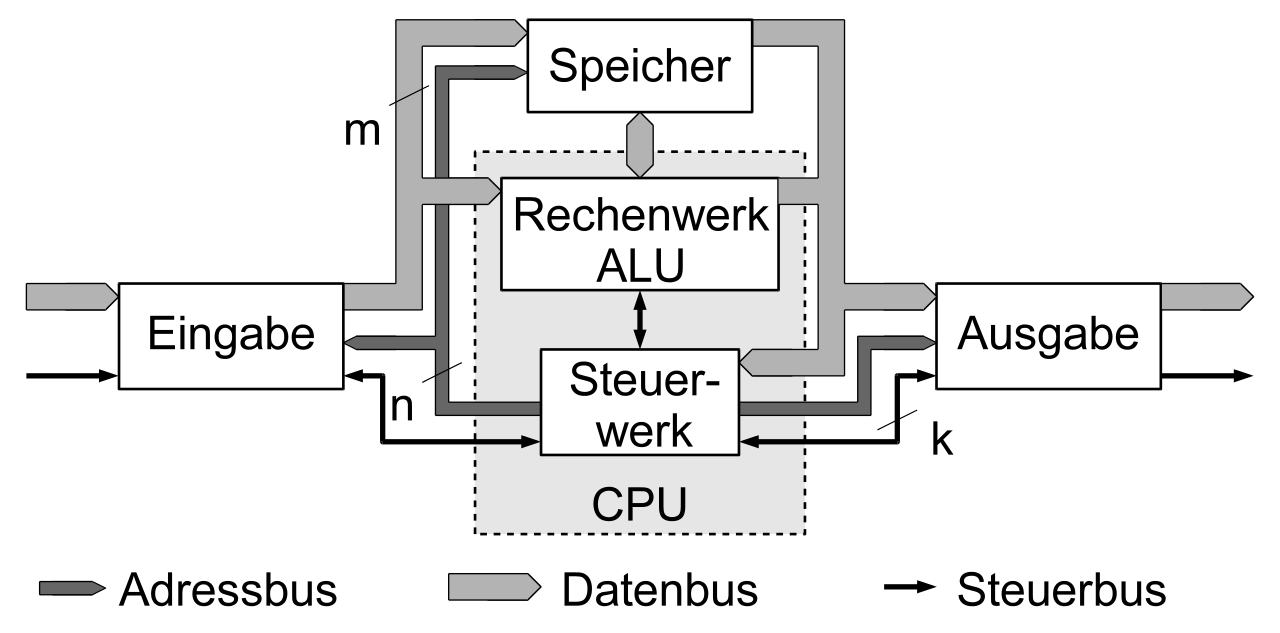
\includegraphics[width=\textwidth]{neumann.png} 
(Medvedev, CC BY-SA 3.0 <https://creativecommons.org/licenses/by-sa/3.0>, via Wikimedia Commons)


% \subsection{$\mu$-Code}

\end{document}
